\documentclass[aspectratio=169,11pt]{beamer}

% ================================================================
% "TABIIY TILNI QAYTA ISHLASH" KURSI
% MA'RUZA 5 --- Ehtimollik modellari: N-gramlar va so'z turkumlari
%              (manba: d05_til_modellari_viz.tex)
% Uslub: 4-ma'ruza (Boadilla + cnublue + defbox/warnbox/okbox)
% 2-haftaning kirish ma'ruzasi; L1-L4 chuqurligi.
% Tayanch qiymat (5-amaliyot birinchi assert): delta(VB,t=2)=0.3402
% ================================================================

% ================================================================
% RANGLAR  (4-ma'ruzadan o'zgarishsiz)
% ================================================================
\definecolor{cnublue}{rgb}{0.07,0.14,0.62}
\definecolor{cnubluelight}{rgb}{0.18,0.30,0.72}
\definecolor{cnubluebg}{rgb}{0.90,0.92,0.97}
\definecolor{deepblue}{rgb}{0.07,0.14,0.62}
\definecolor{deepred}{rgb}{0.60,0.00,0.00}
\definecolor{deepgreen}{rgb}{0.00,0.45,0.00}
\definecolor{halfgray}{gray}{0.55}
\newcommand{\uzq}{\textquotesingle{}}

% ================================================================
% BEAMER MAVZU --- Boadilla + maxsus footer  (4-ma'ruzadan)
% ================================================================
\usetheme{Boadilla}

\setbeamercolor{structure}{fg=cnublue}
\setbeamercolor{frametitle}{bg=cnublue,fg=white}
\setbeamercolor{title}{bg=cnublue,fg=white}
\setbeamercolor{block title}{bg=cnublue,fg=white}
\setbeamercolor{block body}{bg=cnubluebg,fg=black}
\setbeamercolor{alerted text}{fg=deepred}
\setbeamercolor{author in head/foot}{bg=cnubluelight,fg=white}
\setbeamercolor{section in head/foot}{bg=cnublue,fg=white}
\setbeamercolor{page number in head/foot}{bg=cnubluelight,fg=white}

\setbeamertemplate{mini frame}{}
\setbeamertemplate{mini frame in current section}{}
\setbeamertemplate{mini frame in current subsection}{}
\setbeamertemplate{headline}{}
\setbeamertemplate{navigation symbols}{}

\setbeamertemplate{footline}{%
  \leavevmode%
  \hbox{%
    \begin{beamercolorbox}[wd=0.17\paperwidth,ht=2.5ex,dp=1.25ex,leftskip=0.5em]{author in head/foot}%
      \usebeamerfont{author in head/foot}\scriptsize\insertshortauthor%
    \end{beamercolorbox}%
    \begin{beamercolorbox}[wd=0.69\paperwidth,ht=2.5ex,dp=1.25ex,center]{section in head/foot}%
      \usebeamerfont{section in head/foot}%
      \scriptsize\insertsectionnavigationhorizontal{0.69\paperwidth}{}{}%
    \end{beamercolorbox}%
    \begin{beamercolorbox}[wd=0.14\paperwidth,ht=2.5ex,dp=1.25ex,rightskip=0.5em]{page number in head/foot}%
      \hfill\scriptsize\color{white}%
      \insertframenumber{}/\inserttotalframenumber%
    \end{beamercolorbox}%
  }%
  \vskip0pt%
}

% ================================================================
% PAKETLAR  (4-ma'ruzadan + d05 vizualizatsiyalari uchun qo'shimchalar)
% ================================================================
\usepackage[utf8]{inputenc}
\usepackage[T1]{fontenc}
\usepackage{lmodern}
\usepackage{textcomp}
\usepackage{amsmath,amssymb}
\usepackage{booktabs}
\usepackage{xcolor}
\usepackage{listings}
\lstset{
    language=Python,
    basicstyle=\ttfamily\scriptsize,
    keywordstyle=\bfseries\color{deepblue},
    emphstyle=\ttfamily\color{deepred},
    stringstyle=\color{deepgreen},
    commentstyle=\itshape\color{halfgray},
    numbers=none,
    xleftmargin=0pt,
    frame=single,
    framerule=0.4pt,
    rulecolor=\color{cnublue!35},
    columns=fullflexible,
    keepspaces=true,
    breaklines=true,
    breakatwhitespace=false,
    showstringspaces=false,
    tabsize=2
}
\usepackage{tcolorbox}
\tcbuselibrary{skins}
\tcbset{
  defbox/.style={colback=cnubluebg,colframe=cnublue,
                 fonttitle=\small\bfseries\color{white},
                 attach boxed title to top left={yshift=-2mm,xshift=4mm},
                 boxed title style={colback=cnublue,colframe=cnublue}},
  warnbox/.style={colback=orange!8,colframe=orange!70!black,
                  fonttitle=\small\bfseries},
  okbox/.style={colback=green!7,colframe=green!55!black,
                fonttitle=\small\bfseries},
  alertbox/.style={colback=deepred!6,colframe=deepred!75!black,
                   fonttitle=\small\bfseries}
}
\usepackage{tikz}
\usepackage{pgfplots}
\pgfplotsset{compat=1.18}
\usetikzlibrary{arrows.meta,positioning,calc,backgrounds,fit,
                shadows.blur,decorations.pathreplacing,
                shapes.misc,shapes.geometric}

% ================================================================
% VIZUALIZATSIYALAR UCHUN SEMANTIK RANGLAR
% ================================================================
\definecolor{vizorange}{rgb}{0.88,0.46,0.06}
\definecolor{vizgreen}{rgb}{0.00,0.55,0.27}
\definecolor{vizpurple}{rgb}{0.50,0.12,0.55}

\definecolor{NNc}{RGB}{37,71,148}          % NN teg --- ko'k
\definecolor{VBc}{RGB}{200,110,20}         % VB teg --- amber
\definecolor{seenc}{RGB}{37,71,148}        % ko'rilgan
\definecolor{unseenc}{RGB}{176,176,188}    % ko'rilmagan
\definecolor{ForestGreen}{RGB}{28,120,58}
\definecolor{HiRed}{RGB}{197,48,48}
\definecolor{greenbg}{RGB}{233,246,233}
\definecolor{creambg}{RGB}{251,241,222}
\definecolor{brownbar}{RGB}{150,82,20}
\definecolor{greenbar}{RGB}{30,120,55}
\definecolor{bluebg}{RGB}{230,235,250}
\definecolor{mainblue}{rgb}{0.07,0.14,0.62}

% ================================================================
% TikZ STILLARI (d05 izchil vizual tili)
% ================================================================
\tikzset{
  state/.style={circle,draw=black,line width=0.8pt,minimum size=8.5mm,
                font=\small\bfseries,inner sep=0pt},
  nn/.style={state,fill=NNc,text=white},
  vb/.style={state,fill=VBc,text=white},
  obs/.style={rounded corners=2pt,draw=black!55,fill=black!7,
              minimum width=12mm,minimum height=6.5mm,font=\footnotesize\ttfamily},
  wbox/.style={rounded corners=2pt,draw=black!40,fill=black!4,
               minimum width=11mm,minimum height=6mm,font=\footnotesize},
  tran/.style={-{Stealth[length=2.2mm]},line width=0.9pt,NNc!75!black},
  emit/.style={-{Stealth[length=2mm]},dashed,gray!75,line width=0.7pt},
  best/.style={-{Stealth[length=2.8mm]},line width=1.7pt,ForestGreen},
  dep/.style ={-{Stealth[length=2.6mm]},line width=1.3pt,HiRed},
}
% pgfplots: ehtimollik ustun-diagrammasi
\pgfplotsset{
  probbars/.style={
    ybar, bar width=11pt, ymin=0, ymax=1,
    enlarge x limits=0.45, axis y line=left, axis x line=bottom,
    ytick={0,0.5,1}, yticklabel style={font=\scriptsize},
    xtick=data, x tick label style={font=\scriptsize},
    nodes near coords, every node near coord/.append style={font=\scriptsize,anchor=south},
    tick align=outside, clip=false,
  },
}

% ================================================================
% QO'SHIMCHALAR
% ================================================================
\AtBeginSection[]{%
  \begin{frame}{Prezentatsiya rejasi}
    \tableofcontents[currentsection]
  \end{frame}}

% yengil yashil "bajarildi" belgisi (faqat tikz, qo'shimcha paketsiz)
\newcommand{\gcheck}{{\color{ForestGreen}\tikz[baseline=-0.6ex,scale=0.14]{%
  \draw[line width=1.2pt,line cap=round,line join=round](0,0)--(0.45,-0.5)--(1.2,0.65);}}}

% ================================================================
% METAMA'LUMOT
% ================================================================
\title[Ehtimollik modellari]{Ehtimollik modellari: N-grammalar va so\uzq{}z turkumlarini teglash.}
\subtitle{Tabiiy tilni qayta ishlash --- 5-ma\uzq{}ruza}
\author[A.A.\,Abdulali]{A.A.\,Abdulali}
\date{23-iyun 2026}
\institute{11:00--12:20 \quad$\cdot$\quad mavzu \textnumero{}5}


% ================================================================
\begin{document}
% ================================================================

% ----------------------------------------------------------------
% [A] TITUL
% ----------------------------------------------------------------
\maketitle

% ================================================================
\section[Kirish]{Kirish: matnni ehtimollik bilan modellaymiz}
% ================================================================

% ----------------------------------------------------------------
% [B] TAKRORLASH
% ----------------------------------------------------------------
\begin{frame}{Takrorlash: o\uzq{}tgan darslardan ikki savol}
\footnotesize

\begin{columns}[T,totalwidth=\textwidth]
\begin{column}{0.49\textwidth}
\begin{tcolorbox}[warnbox,title=1-savol]
4-ma\uzq{}ruzadagi shovqinli kanal (\textit{noisy channel}) modelida
\[
\hat{w}=\arg\max_w P(x\mid w)\,P(w)
\]
edi. Bu yerdagi til modeli $P(w)$ --- bitta so\uzq{}z ehtimoli ---
\textbf{nechanchi tartibli} N-gram?
\end{tcolorbox}
\end{column}

\begin{column}{0.49\textwidth}
\begin{tcolorbox}[warnbox,title=2-savol]
4-amaliyotda \texttt{edit\_distance} dinamik dasturlash
(\textit{Dynamic Programming, DP}) bilan hisoblangan edi. Bugungi Viterbi ham DP.
Sizningcha, nega ikkalasi ham DP?
\end{tcolorbox}
\end{column}
\end{columns}

\only<2>{
\vspace{3pt}
\begin{columns}[T,totalwidth=\textwidth]
\begin{column}{0.49\textwidth}
\begin{tcolorbox}[okbox,title=1-javob]
Unigram (1-gram) --- so\uzq{}z chastotasi, kontekstsiz.
Bugun uni bigram va trigramga kengaytiramiz, ya\uzq{}ni kontekstni hisobga olamiz.
\end{tcolorbox}
\end{column}

\begin{column}{0.49\textwidth}
\begin{tcolorbox}[okbox,title=2-javob]
Ikkalasi ham masalani kichik qism-masalalarga bo\uzq{}lib, ularning optimal
yechimidan butun yechimni quradi --- bu DP mohiyati.
\end{tcolorbox}
\end{column}
\end{columns}
}

\end{frame}

% ----------------------------------------------------------------
% [C] BUGUNGI MAQSADLAR
% ----------------------------------------------------------------
\begin{frame}{Bugungi dars maqsadlari}
\small

\begin{enumerate}\setlength\itemsep{5pt}
  \item Bigram ehtimolini chastotani sanash asosida
        --- maksimal ehtimollik bahosi (\textit{Maximum Likelihood Estimation, MLE})
        --- zanjir qoidasi (\textit{chain rule}) va Markov taxminidan
        (\textit{Markov assumption}) \textbf{keltirib chiqara olasiz}.

  \item Add-1 (Laplace) silliqlash (\textit{smoothing}) va perplexity (modelning
        matndan \textit{taajjublanish} darajasi) ni kichik korpusda qo\uzq{}lda
        \textbf{hisoblay olasiz}.

  \item Markov zanjiri bilan so\uzq{}z turkumi
        (\textit{Part-of-Speech, POS}) teglari ketma-ketligi ehtimolini
        \textbf{qo\uzq{}llay olasiz}.

  \item Viterbi algoritmini dinamik dasturlash (DP) bilan ishlatib, eng ehtimoliy
        teg ketma-ketligini \textbf{keltirib chiqara olasiz} --- jumladan
        Viterbi jadvalidagi bitta qiymatni qo\uzq{}lda topasiz.
\end{enumerate}

\vspace{4pt}

\begin{tcolorbox}[defbox]
\footnotesize
Oldingi bilimlar: 2-ma\uzq{}ruzadan ehtimollik, $\arg\max$ va logarifm;
4-ma\uzq{}ruzadan dinamik dasturlash va til modeli $P(w)$;
matematikadan ko\uzq{}paytma va maksimum.
\end{tcolorbox}

\end{frame}

% ----------------------------------------------------------------
% [D] REJA VA VAQT BYUDJETI
% ----------------------------------------------------------------
\begin{frame}{Bugungi dars rejasi}
\small
\centering
\renewcommand{\arraystretch}{1.25}
\begin{tabular}{@{}clcl@{}}
\toprule
\textbf{Tsikl} & \textbf{Mavzu}  & \textbf{Natija}\\
\midrule
1  & N-gram til modeli: unigram, bigram, trigram  & $P(\text{kitob}\mid\text{men})=2/3$\\
2  & Laplace silliqlash, keyin perplexity         & add-1 va PP\\
3  & POS teglash va Markov zanjiri                & $P(\mathrm{NN},\mathrm{VB})=0.42$\\
4  & HMM va Viterbi algoritmi                      & $\delta(\mathrm{VB},t{=}2)=0.3402$\\
-- & Xulosa va 5-amaliyotga ko\uzq{}prik           & 5-amaliyot yo\uzq{}nalishi\\
\bottomrule
\end{tabular}

\vspace{6pt}

\begin{tcolorbox}[defbox]
\footnotesize
\textbf{Bu dars 2-haftani ochadi.} Klassik quvurdan (1-hafta) ehtimollik
modellari (2-hafta) ga o\uzq{}tamiz. Bugungi Viterbi qiymati
$\delta(\mathrm{VB},t{=}2)=0.3402$ ertangi 5-amaliyotda \texttt{assert} sifatida tekshiriladi.
Natija ustunidagi sonlar --- soddalashtirilgan o\uzq{}quv misolidan.
\end{tcolorbox}

\end{frame}

% ----------------------------------------------------------------
% [E] MUAMMO BIRINCHI
% ----------------------------------------------------------------
\begin{frame}{Bugungi darsda yechiladigan muammo: \texttt{men \ldots} dan keyin qaysi so\uzq{}z?}
\small

\begin{columns}[T,totalwidth=\textwidth]
\begin{column}{0.50\textwidth}
\textbf{Ikki vazifa}

\begin{tcolorbox}[warnbox,title=1.~Avtomatik to\uzq{}ldirish]
Telefon klaviaturasi \texttt{"men"} dan keyin keyingi so\uzq{}zni taklif qiladi.
Qaysi so\uzq{}z eng ehtimoliy?
\end{tcolorbox}

\vspace{3pt}

\begin{tcolorbox}[warnbox,title=2.~So\uzq{}z turkumini aniqlash]
\texttt{"yozdi"} --- fe\uzq{}lmi yoki ot? Buni kontekst hal qiladi.
Butun gapdagi \textbf{teglar ketma-ketligini} qanday topamiz?
\end{tcolorbox}
\end{column}

\begin{column}{0.46\textwidth}
\textbf{Bugungi yechimlar}

\begin{enumerate}\setlength\itemsep{6pt}
  \item \textbf{N-gram til modeli}: oldingi so\uzq{}z(lar)ga qarab keyingisini
        ehtimollik bilan bashorat qiladi.
  \item \textbf{Yashirin Markov modeli}
        (\textit{Hidden Markov Model, HMM}) \textbf{+ Viterbi}: yashirin teglar
        ketma-ketligining eng ehtimoliysini topadi.
\end{enumerate}

\vspace{4pt}

\begin{tcolorbox}[okbox]
\footnotesize
Ikkala yechimning yuragida bitta g\uzq{}oya: \textbf{ehtimollik} va uni
chastotani sanash asosida baholash.
\end{tcolorbox}
\end{column}
\end{columns}

\end{frame}

% ================================================================
\section[N-gram]{N-gram til modellari}
% ================================================================

% ----------------------------------------------------------------
% [F1] INTUITSIYA: kontekst oynasi
% ----------------------------------------------------------------
\begin{frame}{Intuitsiya: keyingi so\uzq{}zni oldingilariga qarab bashorat qilamiz}
\footnotesize

\begin{columns}[T,totalwidth=\textwidth]
\begin{column}{0.44\textwidth}
\texttt{"men"} $\rightarrow$ \texttt{kitob}? \texttt{non}? \texttt{keldim}?

\vspace{3pt}
Til modeli (\textit{language model}) har bir davom uchun \textbf{ehtimol} beradi
va eng yuqorisini taklif qiladi.

\vspace{5pt}
\textbf{Nechta oldingi so\uzq{}z hisobga olinadi?}
\begin{itemize}\setlength\itemsep{3pt}
  \item \textbf{unigram}: kontekstsiz --- $P(w)$
  \item \textbf{bigram}: 1 oldingi --- $P(w_i\mid w_{i-1})$
  \item \textbf{trigram}: 2 oldingi --- $P(w_i\mid w_{i-2},w_{i-1})$
\end{itemize}
\end{column}

\begin{column}{0.54\textwidth}
\centering
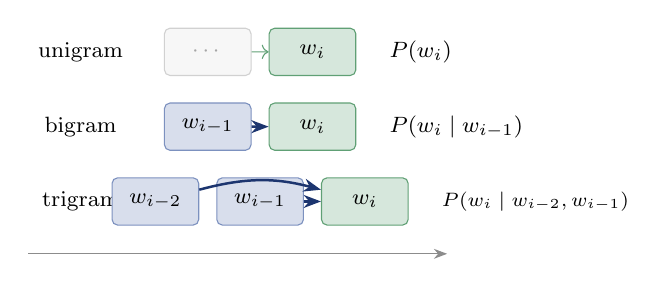
\begin{tikzpicture}[font=\footnotesize,scale=0.95,
    ctx/.style={wbox,fill=NNc!18,draw=NNc!60},
    tgt/.style={wbox,fill=ForestGreen!18,draw=ForestGreen!70},
    ghost/.style={wbox,draw=black!18,fill=black!3,text=black!35}]
  % unigram
  \node at (-1.7,2.0) {unigram};
  \node[ghost] (u1) at (0.0,2.0) {$\cdots$};
  \node[tgt]   (ut) at (1.4,2.0) {$w_i$};
  \draw[->,ForestGreen!70] (u1) -- (ut);
  \node[anchor=west] at (2.3,2.0) {$P(w_i)$};
  % bigram
  \node at (-1.7,1.0) {bigram};
  \node[ctx] (b1) at (0.0,1.0) {$w_{i-1}$};
  \node[tgt] (bt) at (1.4,1.0) {$w_i$};
  \draw[tran] (b1) -- (bt);
  \node[anchor=west] at (2.3,1.0) {$P(w_i\mid w_{i-1})$};
  % trigram
  \node at (-1.7,0.0) {trigram};
  \node[ctx] (t1) at (-0.7,0.0) {$w_{i-2}$};
  \node[ctx] (t2) at ( 0.7,0.0) {$w_{i-1}$};
  \node[tgt] (tt) at ( 2.1,0.0) {$w_i$};
  \draw[tran] (t2) -- (tt);
  \draw[tran,bend left=15] (t1) to (tt);
  \node[anchor=west] at (3.0,0.0) {\scriptsize$P(w_i\mid w_{i-2},w_{i-1})$};
  % kontekst o'qi
  \draw[-{Stealth},black!45] (-2.4,-0.7) -- (3.2,-0.7);
\end{tikzpicture}

\vspace{4pt}

\begin{tcolorbox}[okbox,left=2mm,right=2mm,top=1mm,bottom=1mm]
\scriptsize
Ko\uzq{}proq kontekst $\Rightarrow$ aniqroq bashorat, lekin ko\uzq{}proq ma\uzq{}lumot
kerak (kam uchraydigan N-gramlar). Bu murosani 2-tsiklda ko\uzq{}ramiz.
\end{tcolorbox}
\end{column}
\end{columns}

\end{frame}

% ----------------------------------------------------------------
% [G1] RASMIY TA'RIF: N-gram + normalizatsiya viz
% ----------------------------------------------------------------
\begin{frame}{N-gram til modeli: rasmiy ta\uzq{}rif}
\footnotesize

\begin{columns}[T,totalwidth=\textwidth]
%------------------------------------------------
\begin{column}{0.53\textwidth}

\begin{tcolorbox}[defbox,left=2mm,right=2mm,top=1mm,bottom=1mm]
\[
P(w_i\mid w_{i-1})
=
\frac{\operatorname{count}(w_{i-1},w_i)}
{\operatorname{count}(w_{i-1})}
\]
\end{tcolorbox}

\vspace{2pt}

\[
\operatorname{count}(w_{i-1},w_i)
\]
{\scriptsize $w_{i-1}$ dan keyin $w_i$ kelgan hollar soni.}

\vspace{3pt}

\textbf{MLE} (\textit{Maximum Likelihood Estimation}) — chastotaga asoslangan baho.

\vspace{5pt}

\textbf{Gap ehtimoli (bigram):}
\[
P(w_1,\ldots,w_n)
\approx
\prod_{i=1}^{n+1}P(w_i\mid w_{i-1})
\]

\[
w_0=\langle s\rangle,\qquad
w_{n+1}=\langle/s\rangle
\]

{\scriptsize $\langle s\rangle$ — gap boshi, $\langle/s\rangle$ — gap oxiri.}

\vspace{4pt}

\begin{tcolorbox}[defbox,left=2mm,right=2mm,top=1mm,bottom=1mm]
\scriptsize
Trigramda kontekst ikki so\uzq{}zdan iborat bo\uzq{}ladi:
\[
P(w_i\mid w_{i-2},w_{i-1}).
\]
\end{tcolorbox}

\end{column}

%------------------------------------------------
\begin{column}{0.43\textwidth}
\centering

\textbf{\scriptsize Misol: \texttt{men} dan keyingi so\uzq{}zlar}

\vspace{2pt}

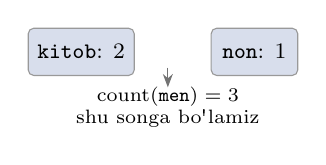
\begin{tikzpicture}[font=\scriptsize]
  \node[wbox,fill=NNc!18] (ck) at (-1.1,1.15) {\texttt{kitob}: 2};
  \node[wbox,fill=NNc!18] (cn) at ( 1.1,1.15) {\texttt{non}: 1};

  \node[align=center] at (0,0.45)
  {$\operatorname{count}(\texttt{men})=3$\\
   shu songa bo\uzq{}lamiz};

  \draw[-{Stealth},black!55] (0,0.95) -- (0,0.70);
\end{tikzpicture}

\vspace{-3pt}

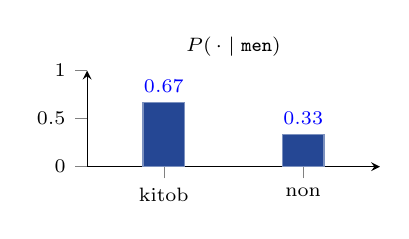
\begin{tikzpicture}
  \begin{axis}[
      probbars,
      bar shift=0pt,
      enlarge x limits=0.55,
      width=5.3cm,
      height=2.8cm,
      symbolic x coords={kitob,non},
      bar width=15pt,
      title={\scriptsize $P(\,\cdot\mid\texttt{men})$},
      title style={yshift=-1ex}
    ]
    \addplot+[fill=seenc,draw=seenc!60]
      coordinates {(kitob,0.667) (non,0.333)};
  \end{axis}
\end{tikzpicture}

\vspace{1pt}

\begin{tcolorbox}[okbox,left=2mm,right=2mm,top=1mm,bottom=1mm]
\scriptsize
\[
P(\texttt{kitob}\mid\texttt{men})=\frac{2}{3}\approx0.67
\]
\[
P(\texttt{non}\mid\texttt{men})=\frac{1}{3}\approx0.33
\]
\end{tcolorbox}

\end{column}
\end{columns}

\end{frame}
% ----------------------------------------------------------------
% [G1b] MAXSUS TOKENLAR
% ----------------------------------------------------------------
\begin{frame}{Amaliy eslatma: gap chegaralari va maxsus tokenlar}
\footnotesize

\begin{columns}[T,totalwidth=\textwidth]
\begin{column}{0.55\textwidth}
N-gram modelda gap boshi va oxiri ham hisobga olinadi. Shunda birinchi
so\uzq{}z ham ehtimollik oladi:
\[
P(\text{men}\mid \langle s\rangle).
\]
Gap oxiri $\langle /s\rangle$ ham zarur: usiz model qisqa gaplarga moyil
bo\uzq{}ladi va ehtimollar taqsimoti noto\uzq{}liq qoladi.

\vspace{6pt}
\centering
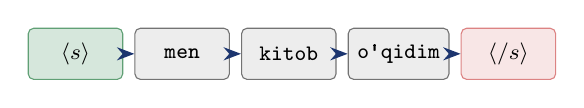
\begin{tikzpicture}[font=\footnotesize,node distance=4pt]
  \node[obs,fill=ForestGreen!18,draw=ForestGreen!70] (s)  {$\langle s\rangle$};
  \node[obs,right=of s] (w1) {men};
  \node[obs,right=of w1] (w2) {kitob};
  \node[obs,right=of w2] (w3) {o\uzq{}qidim};
  \node[obs,right=of w3,fill=HiRed!12,draw=HiRed!60] (e) {$\langle/s\rangle$};

  \draw[tran] (s)  -- (w1);
  \draw[tran] (w1) -- (w2);
  \draw[tran] (w2) -- (w3);
  \draw[tran] (w3) -- (e);

\end{tikzpicture}
\end{column}

\begin{column}{0.45\textwidth}
\begin{tcolorbox}[okbox,left=2mm,right=2mm,top=1mm,bottom=1mm]
\scriptsize
\textbf{O\uzq{}zbek matni uchun.} Apostrof, tire, raqam va qo\uzq{}shimchalar
normallashtirilmasa, sanoqlar sun\uzq{}iy bo\uzq{}linib ketadi:
\texttt{o\uzq{}qidim} va \texttt{o qidim} ikki xil token bo\uzq{}lib qolishi mumkin.
\end{tcolorbox}

\vspace{4pt}
Amalda gap boshi \texttt{<s>}, gap oxiri \texttt{</s>} va noma\uzq{}lum
so\uzq{}z \texttt{<UNK>} (\textit{unknown}) belgilari izchil qo\uzq{}llanadi.
\end{column}
\end{columns}

\end{frame}

% ----------------------------------------------------------------
% [H1] KELTIRIB CHIQARISH: zanjir -> bigram  (statik)
% ----------------------------------------------------------------
\begin{frame}{Keltirib chiqarish: zanjir qoidasidan bigramga}
\footnotesize

\textbf{1-qadam.} Zanjir qoidasi (\textit{chain rule}) --- ehtimolliklar ko\uzq{}paytmasi:
\[
P(w_1,\dots,w_n)=\prod_{i=1}^{n} P(w_i\mid w_1,\dots,w_{i-1})
\]

\vspace{2pt}
\textbf{2-qadam.} Muammo: bunday uzun kontekstlar kam uchraydi, shuning uchun
ularni ishonchli sanash qiyin.

\vspace{2pt}
\textbf{3-qadam.} \textbf{Markov taxmini} (\textit{Markov assumption}):
faqat oxirgi $n-1$ ta so\uzq{}z muhim deb olinadi. Bigramda bu:
\[
P(w_i\mid w_1,\dots,w_{i-1}) \approx P(w_i\mid w_{i-1})
\]

\vspace{6pt}

\begin{center}
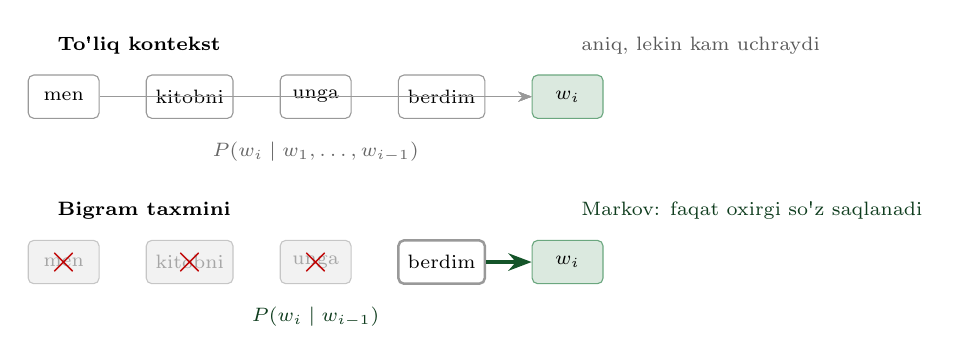
\begin{tikzpicture}[
    font=\scriptsize,
    wb/.style={draw, rounded corners=2pt, minimum width=9mm, minimum height=5.5mm, align=center},
    keep/.style={wb, fill=ForestGreen!16, draw=ForestGreen!65},
    gone/.style={wb, fill=gray!10, draw=gray!45, text=gray!70},
    norm/.style={wb, fill=white, draw=black!40},
    >=Stealth
  ]

  % Yuqori qator: to'liq kontekst
  \node[anchor=west,font=\scriptsize\bfseries] at (-0.2,1.55) {To\uzq{}liq kontekst};
  \node[anchor=west,font=\scriptsize,text=black!65] at (6.45,1.55) {aniq, lekin kam uchraydi};

  \node[norm] (a1) at (0,0.9) {men};
  \node[norm] (a2) at (1.6,0.9) {kitobni};
  \node[norm] (a3) at (3.2,0.9) {unga};
  \node[norm] (a4) at (4.8,0.9) {berdim};
  \node[keep] (a5) at (6.4,0.9) {$w_i$};

  \foreach \u in {a1,a2,a3,a4}{
    \draw[->,black!40] (\u) -- (a5);
  }

  \node[align=center,font=\scriptsize,text=black!60] at (3.2,0.2)
  {$P(w_i \mid w_1,\dots,w_{i-1})$};

  % Pastki qator: bigram Markov taxmini
  \node[anchor=west,font=\scriptsize\bfseries] at (-0.2,-0.55) {Bigram taxmini};
  \node[anchor=west,font=\scriptsize,text=ForestGreen!50!black] at (6.45,-0.55)
  {Markov: faqat oxirgi so\uzq{}z saqlanadi};

  \node[gone] (b1) at (0,-1.2) {men};
  \node[gone] (b2) at (1.6,-1.2) {kitobni};
  \node[gone] (b3) at (3.2,-1.2) {unga};
  \node[norm, line width=0.9pt] (b4) at (4.8,-1.2) {berdim};
  \node[keep] (b5) at (6.4,-1.2) {$w_i$};

  % E'tibordan chiqarilgan kontekstlar
  \node[text=red!75!black,font=\Large] at (0,-1.2) {$\times$};
  \node[text=red!75!black,font=\Large] at (1.6,-1.2) {$\times$};
  \node[text=red!75!black,font=\Large] at (3.2,-1.2) {$\times$};

  % Faqat oxirgi so'z saqlanadi
  \draw[->,line width=1.2pt,ForestGreen!70!black] (b4) -- (b5);

  \node[align=center,font=\scriptsize,text=ForestGreen!50!black] at (3.2,-1.9)
  {$P(w_i \mid w_{i-1})$};

\end{tikzpicture}
\end{center}

\end{frame}

% ----------------------------------------------------------------
% [I1] QO'LDA MISOL: bigram
% ----------------------------------------------------------------
\begin{frame}{Qo\uzq{}lda misol: bigram ehtimolini sanaymiz}
\footnotesize

\begin{tcolorbox}[defbox,left=2mm,right=2mm,top=1mm,bottom=1mm]
\scriptsize
Korpus: \;\;S1: men kitob o\uzq{}qidim \quad S2: men non yedim \quad S3: men kitob oldim
\end{tcolorbox}

\vspace{4pt}

\begin{columns}[T,totalwidth=\textwidth]
\begin{column}{0.50\textwidth}
\textbf{Sanaymiz}
\[
\operatorname{count}(\text{men})=3,\qquad
\operatorname{count}(\text{men},\text{kitob})=2
\]
\[
P(\text{kitob}\mid\text{men})=\tfrac{2}{3}\approx 0.667
\]

\vspace{3pt}
Lug\uzq{}at hajmi $|V|=6$:
men, kitob, o\uzq{}qidim, non, yedim, oldim.
\end{column}

\begin{column}{0.46\textwidth}
\centering
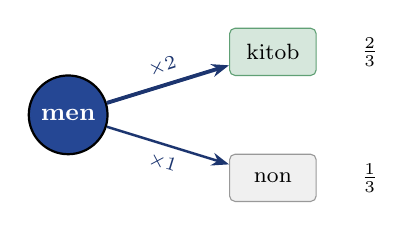
\begin{tikzpicture}[font=\footnotesize]
  \node[state,fill=NNc,text=white,minimum size=10mm] (men) at (0,0) {men};
  \node[wbox,fill=ForestGreen!18,draw=ForestGreen!70] (k) at (2.6,0.8) {kitob};
  \node[wbox,fill=black!6] (n) at (2.6,-0.8) {non};
  \draw[tran,line width=1.4pt] (men) to node[above,sloped]{\scriptsize $\times 2$} (k);
  \draw[tran] (men) to node[below,sloped]{\scriptsize $\times 1$} (n);
  \node[anchor=west] at (3.6,0.8) {$\tfrac{2}{3}$};
  \node[anchor=west] at (3.6,-0.8) {$\tfrac{1}{3}$};
\end{tikzpicture}

\vspace{3pt}
\begin{tcolorbox}[okbox,left=2mm,right=2mm,top=1mm,bottom=1mm]
\scriptsize
``men'' dan keyin \texttt{kitob} (2 marta) \texttt{non} (1 marta) dan ko\uzq{}proq
kutiladi $\Rightarrow$ avtomatik to\uzq{}ldirish \texttt{kitob} ni taklif qiladi.
\end{tcolorbox}
\end{column}
\end{columns}

\end{frame}

% ----------------------------------------------------------------
% [J1] SIZNING VAZIFANGIZ: P(non|men)   (2 betli overlay)
% ----------------------------------------------------------------
\begin{frame}{Sizning vazifangiz: yana bir bigram}
\small

\only<1>{
\begin{tcolorbox}[warnbox,title=Vazifa]
Xuddi shu korpus (S1, S2, S3) uchun:
\[
P(\text{non}\mid\text{men})=\,?
\]
\end{tcolorbox}
}

\only<2>{
\begin{columns}[T,totalwidth=\textwidth]
\begin{column}{0.52\textwidth}
\begin{tcolorbox}[warnbox,title=Vazifa]
\[
P(\text{non}\mid\text{men})=\,?
\]
\end{tcolorbox}

\vspace{3pt}
\begin{tcolorbox}[okbox,title=Javob]
\footnotesize
$\operatorname{count}(\text{men},\text{non})=1,\ \operatorname{count}(\text{men})=3$
\[
P(\text{non}\mid\text{men})=\tfrac{1}{3}\approx 0.333
\]
Tekshiruv: $\tfrac{2}{3}+\tfrac{1}{3}=1$ --- ``men'' dan keyin faqat shu ikki so\uzq{}z kelgan.
\end{tcolorbox}
\end{column}

\begin{column}{0.44\textwidth}
\centering
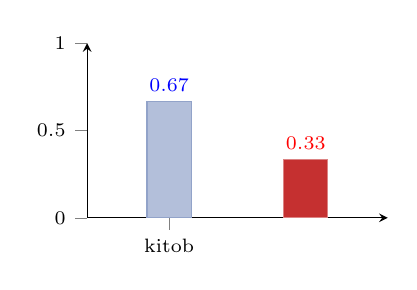
\begin{tikzpicture}
  \begin{axis}[probbars, bar shift=0pt, enlarge x limits=0.6, width=5.4cm, height=3.8cm,
      symbolic x coords={kitob,non}, bar width=16pt]
    \addplot+[fill=seenc!35,draw=seenc!50] coordinates {(kitob,0.667)};
    \addplot+[fill=HiRed,draw=HiRed!60] coordinates {(non,0.333)};
  \end{axis}
\end{tikzpicture}\\[-2pt]
{\scriptsize yig\uzq{}indi $=1$ $\checkmark$}
\end{column}
\end{columns}
}

\end{frame}

% ----------------------------------------------------------------
% [K1] KOD <-> FORMULA: bigram  [fragile]
% ----------------------------------------------------------------
\begin{frame}[fragile]{Kod va formula: bigram modeli}
\scriptsize

\begin{columns}[T,totalwidth=\textwidth]
\begin{column}{0.58\textwidth}
\textbf{Python kodi}

\begin{tcolorbox}[defbox,left=2mm,right=2mm,top=1mm,bottom=1mm]
\begin{verbatim}
from collections import Counter
corpus = [["men","kitob","o'qidim"],
          ["men","non","yedim"],
          ["men","kitob","oldim"]]
uni = Counter(w for s in corpus for w in s)
bi  = Counter((s[i], s[i+1])
              for s in corpus
              for i in range(len(s)-1))

def p_bigram(prev, w):
    return bi[(prev, w)] / uni[prev]

p = p_bigram("men", "kitob")
print(round(p, 3))   # 0.667
\end{verbatim}
\end{tcolorbox}
\end{column}

\begin{column}{0.40\textwidth}
\textbf{Kod va formula mosligi}

\begin{tabular}{@{}l l@{}}
\toprule
\textbf{Kod} & \textbf{Formula} \\
\midrule
\texttt{bi[(prev,w)]} & $\operatorname{count}(w_{i-1},w_i)$ \\
\texttt{uni[prev]}    & $\operatorname{count}(w_{i-1})$ \\
\texttt{bi/uni}       & $P(w_i\mid w_{i-1})$ \\
\bottomrule
\end{tabular}

\vspace{6pt}

\begin{tcolorbox}[okbox,left=2mm,right=2mm,top=1mm,bottom=1mm]
\scriptsize
Ertangi 5-amaliyotdagi \texttt{m05 Autocomplete} moduli aynan shu sanashga tayanadi.
\end{tcolorbox}
\end{column}
\end{columns}

\end{frame}

% ----------------------------------------------------------------
% [L1] CHEKLOV: zero problem
% ----------------------------------------------------------------
\begin{frame}{N-gram tuzog\uzq{}i: ko\uzq{}rilmagan birikma butun gapni nolga aylantiradi}
\footnotesize

\begin{columns}[T,totalwidth=\textwidth]
\begin{column}{0.46\textwidth}
\begin{tcolorbox}[warnbox,title=Nol muammosi (\textit{zero problem})]
Test gapi: \texttt{"men non o'qidim"}.

\vspace{2pt}
\texttt{(non, o'qidim)} korpusda hech uchramagan $\Rightarrow P=0$.

\vspace{3pt}
Bigram ko\uzq{}paytmada bitta $0$ $\Rightarrow$ \textbf{butun gap ehtimoli} $=0$.
\end{tcolorbox}
\end{column}

\begin{column}{0.54\textwidth}
\centering
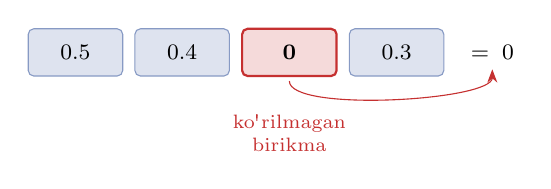
\begin{tikzpicture}[font=\footnotesize,
    f/.style={wbox,minimum width=12mm,fill=NNc!15,draw=NNc!55}]
  \node[f] (a) {0.5};
  \node[f,right=4pt of a] (b) {0.4};
  \node[f,right=4pt of b,fill=HiRed!18,draw=HiRed,thick] (c) {\textbf{0}};
  \node[f,right=4pt of c] (d) {0.3};
  \node[right=6pt of d] (eq) {$=\;0$};
  \node[below=10pt of c,HiRed,align=center] {\scriptsize ko\uzq{}rilmagan\\[-1pt]\scriptsize birikma};
  \draw[-{Stealth},HiRed] ($(c.south)+(0,-0.05)$) .. controls +(0,-0.4) and +(0,-0.4) .. (eq.south);
\end{tikzpicture}

\vspace{6pt}
\begin{tcolorbox}[okbox,left=2mm,right=2mm,top=1mm,bottom=1mm]
\scriptsize
Model ko\uzq{}rmagan birikmani ``imkonsiz'' deb hisoblaydi --- til esa cheksiz ijodiy.
\textbf{2-tsikl ikki qadam:} (1) \textbf{silliqlash} nol muammosini hal qiladi;
(2) keyin tayyor modelni \textbf{perplexity} bilan baholaymiz.
\end{tcolorbox}
\end{column}
\end{columns}

\end{frame}

% ================================================================
\section[Silliqlash]{Silliqlash va perplexity}
% ================================================================

% ----------------------------------------------------------------
% [F2] perplexity intuitsiya+ta'rif ---> silliqlash blokidan KEYIN ko'chirildi
%      (oqim: avval silliqlash nol muammosini hal qiladi, keyin perplexity baholaydi)
% ----------------------------------------------------------------
% ----------------------------------------------------------------
% [G2] RASMIY: add-1 silliqlash  (perplexity blokga ko'chirildi)
% ----------------------------------------------------------------
\begin{frame}{Add-1 (Laplace) silliqlash: ta\uzq{}rif}
\footnotesize

\begin{columns}[T,totalwidth=\textwidth]
\begin{column}{0.52\textwidth}
\textbf{Nol muammosi yodimizda:} ko\uzq{}rilmagan birikma $\Rightarrow P=0$.
Eng oddiy yechim --- har bigram sanog\uzq{}iga $+1$ (\textit{add-1 / Laplace}):
\begin{tcolorbox}[defbox,left=2mm,right=2mm,top=1mm,bottom=1mm]
\footnotesize
\[
P_{+1}(w_i\mid w_{i-1})=\frac{\operatorname{count}(w_{i-1},w_i)+1}{\operatorname{count}(w_{i-1})+|V|}
\]
\end{tcolorbox}

\vspace{6pt}
Ko\uzq{}rilgan birikmalardan ehtimollik massasining bir qismi
ko\uzq{}rilmaganlarga \textbf{ko\uzq{}chadi} --- model ``yangilik''ka tayyor bo\uzq{}ladi.
Maxrajdagi $|V|$ ning sababini keyingi slaydda chiqaramiz.
\end{column}

\begin{column}{0.48\textwidth}
\centering
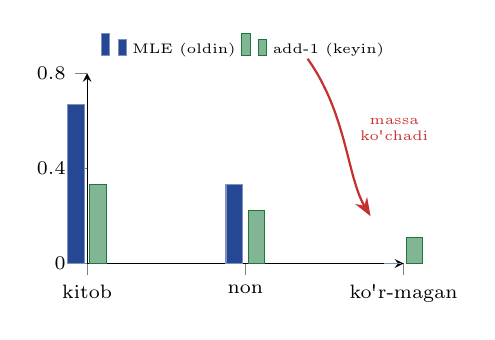
\begin{tikzpicture}
  \begin{axis}[
      ybar, bar width=6pt, width=5.6cm, height=4.0cm,
      ymin=0, ymax=0.8, enlarge x limits=0.28,
      symbolic x coords={kitob,non,kormagan}, xtick=data,
      xticklabels={kitob,non,{ko\uzq{}r-magan}},
      x tick label style={font=\scriptsize}, yticklabel style={font=\scriptsize},
      ytick={0,0.4,0.8},
      legend style={font=\tiny,at={(0.5,1.02)},anchor=south,legend columns=2,draw=none},
      axis y line=left, axis x line=bottom, tick align=outside, clip=false]
    \addplot+[fill=seenc,draw=seenc!60] coordinates {(kitob,0.667)(non,0.333)(kormagan,0)};
    \addplot+[fill=ForestGreen!55,draw=ForestGreen] coordinates {(kitob,0.333)(non,0.222)(kormagan,0.111)};
    \legend{MLE (oldin),add-1 (keyin)}
  \end{axis}
  \draw[-{Stealth},HiRed,thick] (2.8,2.6) .. controls (3.3,1.9) and (3.3,1.1) .. (3.6,0.6);
  \node[HiRed,font=\tiny,align=center] at (3.9,1.7) {massa\\ ko\uzq{}chadi};
\end{tikzpicture}\\[-1pt]
{\scriptsize ko\uzq{}rilgan $\downarrow$, ko\uzq{}rilmagan $0\!\to\!{>}0$}
\end{column}
\end{columns}

\end{frame}

% ----------------------------------------------------------------
% [H2] KELTIRIB CHIQARISH: nega |V|  (statik)
% ----------------------------------------------------------------
\begin{frame}{Keltirib chiqarish: nega maxrajga $|V|$ qo\uzq{}shamiz?}
\footnotesize

\textbf{1-qadam.} Har bigram sanog\uzq{}iga $+1$ qo\uzq{}shamiz; shunda ko\uzq{}rilmaganlar
ham $0$ emas, $1$ bo\uzq{}ladi.

\textbf{2-qadam.} Ehtimollar yig\uzq{}indisi $1$ bo\uzq{}lishi shart. $w_{i-1}$ dan keyin
har bir lug\uzq{}at so\uzq{}zi ($|V|$ ta) uchun $+1$ qo\uzq{}shdik:
\[
\sum_{w}\big(\operatorname{count}(w_{i-1},w)+1\big)=\operatorname{count}(w_{i-1})+|V|
\]

\textbf{3-qadam.} Shuning uchun maxraj $\operatorname{count}(w_{i-1})+|V|$.

\vspace{2pt}
\begin{center}
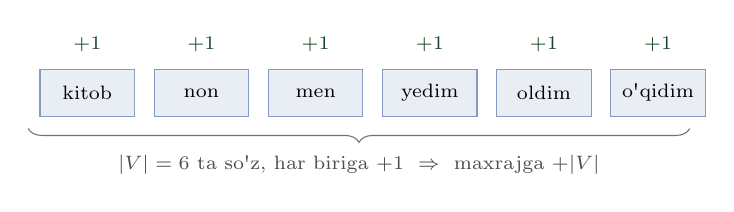
\begin{tikzpicture}[font=\scriptsize,cell/.style={draw=NNc!55,fill=NNc!10,minimum width=12mm,minimum height=6mm}]
  \foreach \i/\lab in {1/{kitob},2/{non},3/{men},4/{yedim},5/{oldim},6/{o\uzq{}qidim}}{
    \node[cell] (c\i) at (\i*1.45,0) {\lab};
    \node[ForestGreen!60!black] at (\i*1.45,0.62) {\scriptsize $+1$};}
  \draw[decorate,decoration={brace,amplitude=5pt,mirror},black!55]
    (0.7,-0.45) -- (9.1,-0.45)
    node[midway,below=6pt,black!70]{$|V|=6$ ta so\uzq{}z, har biriga $+1$ $\;\Rightarrow\;$ maxrajga $+|V|$};
\end{tikzpicture}
\end{center}

\end{frame}

% ----------------------------------------------------------------
% [I2] QO'LDA MISOL: silliqlash nolni hal qiladi
% ----------------------------------------------------------------
\begin{frame}{Qo\uzq{}lda misol: silliqlash nol muammosini hal qiladi}
\footnotesize

\begin{columns}[T,totalwidth=\textwidth]
\begin{column}{0.50\textwidth}
$|V|=6,\ \operatorname{count}(\text{non})=1,\ \operatorname{count}(\text{non},\text{o\uzq{}qidim})=0$.

\vspace{6pt}
Silliqlashsiz:
\[
P(\text{o\uzq{}qidim}\mid\text{non})=\tfrac{0}{1}=0\ \Rightarrow\ \text{gap ehtimoli}=0
\]

\vspace{2pt}
Add-1 bilan:
\[
P_{+1}(\text{o\uzq{}qidim}\mid\text{non})=\tfrac{0+1}{1+6}=\tfrac{1}{7}\approx 0.143
\]
\end{column}

\begin{column}{0.48\textwidth}
\centering
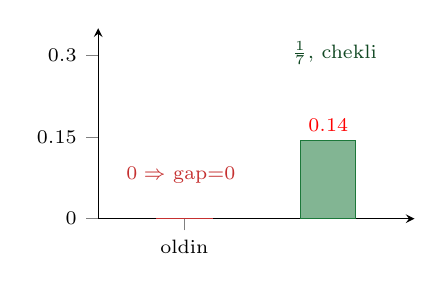
\begin{tikzpicture}
  \begin{axis}[probbars, bar shift=0pt, enlarge x limits=0.6, width=5.6cm, height=4.0cm, ymax=0.35, ytick={0,0.15,0.3},
      symbolic x coords={oldin,keyin}, bar width=20pt]
    \addplot+[fill=HiRed!30,draw=HiRed,nodes near coords={}] coordinates {(oldin,0.001)};
    \addplot+[fill=ForestGreen!55,draw=ForestGreen] coordinates {(keyin,0.143)};
  \end{axis}
  \node[HiRed,font=\scriptsize] at (1.05,0.55) {$0\Rightarrow$ gap${=}0$};
  \node[ForestGreen!60!black,font=\scriptsize] at (3.0,2.1) {$\tfrac{1}{7}$, chekli};
\end{tikzpicture}\\[-1pt]
{\scriptsize Silliqlash modelni ``yangilik''ka tayyor qiladi.}
\end{column}
\end{columns}

\end{frame}

% ----------------------------------------------------------------
% [J2] SIZNING VAZIFANGIZ: P+1(kitob|men)   (2 betli overlay)
% ----------------------------------------------------------------
\begin{frame}{Sizning vazifangiz: add-1 ehtimolini hisoblang}
\small

\only<1>{
\begin{tcolorbox}[warnbox,title=Vazifa]
$|V|=6,\ \operatorname{count}(\text{men})=3,\ \operatorname{count}(\text{men},\text{kitob})=2$:
\[
P_{+1}(\text{kitob}\mid\text{men})=\,?
\]
Silliqlashsiz qiymat $2/3$ edi --- add-1 dan keyin qanday o\uzq{}zgaradi?
\end{tcolorbox}
}

\only<2>{
\begin{columns}[T,totalwidth=\textwidth]
\begin{column}{0.54\textwidth}
\begin{tcolorbox}[warnbox,title=Vazifa]
\[
P_{+1}(\text{kitob}\mid\text{men})=\,?
\]
\end{tcolorbox}

\vspace{3pt}
\begin{tcolorbox}[okbox,title=Javob]
\footnotesize
\[
P_{+1}(\text{kitob}\mid\text{men})=\frac{2+1}{3+6}=\frac{3}{9}=\tfrac13\approx 0.333
\]
Ko\uzq{}rilgan birikma ehtimoli $2/3\to 1/3$ ga pasaydi --- massa ko\uzq{}rilmaganlarga
ko\uzq{}chdi. Bu silliqlash narxi.
\end{tcolorbox}
\end{column}

\begin{column}{0.44\textwidth}
\centering
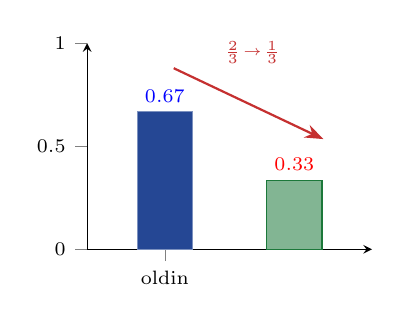
\begin{tikzpicture}
  \begin{axis}[probbars, bar shift=0pt, enlarge x limits=0.6, width=5.2cm, height=4.2cm, ymax=1.0, ytick={0,0.5,1},
      symbolic x coords={oldin,keyin}, bar width=20pt]
    \addplot+[fill=seenc,draw=seenc!60] coordinates {(oldin,0.667)};
    \addplot+[fill=ForestGreen!55,draw=ForestGreen] coordinates {(keyin,0.333)};
  \end{axis}
  \draw[-{Stealth},HiRed,thick] (1.1,2.3) -- (3.0,1.4);
  \node[HiRed,font=\tiny] at (2.1,2.5) {$\tfrac23\!\to\!\tfrac13$};
\end{tikzpicture}
\end{column}
\end{columns}
}

\end{frame}

% ----------------------------------------------------------------
% [F2'] PERPLEXITY: intuitsiya + ta'rif  (silliqlashdan KEYIN)
% ----------------------------------------------------------------
\begin{frame}{Perplexity: modelning noaniqlik darajasi}
\footnotesize

\begin{columns}[T,totalwidth=\textwidth]
%------------------------------------------------
\begin{column}{0.52\textwidth}

\textbf{Perplexity (PP) nima?}

\vspace{2pt}
Perplexity — model test matnini ko\uzq{}rganda qanchalik
noaniq qaror qilayotganini ko\uzq{}rsatadigan baholash mezoni.

\vspace{3pt}

\begin{itemize}\setlength\itemsep{4pt}
  \item \textbf{Past PP} — model keyingi tokenlarni yaxshi kutgan.
  \item \textbf{Yuqori PP} — model ko\uzq{}p variant orasida noaniq qolgan.
\end{itemize}

\vspace{4pt}

\begin{tcolorbox}[defbox,left=2mm,right=2mm,top=1mm,bottom=1mm]
\[
\mathrm{PP}(W)
=
\exp\!\left(
-\frac{1}{N}
\sum_{i=1}^{N}
\ln P(w_i\mid w_{i-1})
\right)
\]
\end{tcolorbox}

\vspace{2pt}

{\scriptsize
$N$ — test matndagi tokenlar soni.  
Bigram modelda har bir token ehtimoli oldingi token orqali baholanadi.
}

\end{column}

%------------------------------------------------
\begin{column}{0.44\textwidth}
\centering

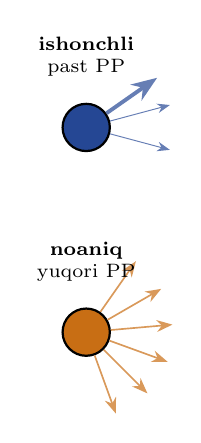
\begin{tikzpicture}[font=\scriptsize]
  % low PP
  \node[state,fill=NNc,text=white,minimum size=6mm] (c) at (0,1.35) {};
  \foreach \a/\w in {35/1.4pt,15/0.35pt,-15/0.35pt}
    \draw[-{Stealth},line width=\w,NNc!70] (c) -- ++(\a:1.1);
  \node[align=center] at (0,2.25)
    {\textbf{ishonchli}\\ past PP};

  % high PP
  \node[state,fill=VBc,text=white,minimum size=6mm] (d) at (0,-1.25) {};
  \foreach \a in {55,30,5,-20,-45,-70}
    \draw[-{Stealth},line width=0.6pt,VBc!70] (d) -- ++(\a:1.1);
  \node[align=center] at (0,-0.35)
    {\textbf{noaniq}\\ yuqori PP};
\end{tikzpicture}

\vspace{4pt}

\begin{tcolorbox}[okbox,left=2mm,right=2mm,top=1mm,bottom=1mm]
\scriptsize
PP taxminan model har qadamda nechta teng ehtimolli variant
orasidan tanlayotgandek ekanini bildiradi.
\end{tcolorbox}

\vspace{3pt}

\[
\text{PP past} \Rightarrow \text{model yaxshiroq}
\]

\end{column}
\end{columns}

\end{frame}

% ----------------------------------------------------------------
% [K2] KOD <-> FORMULA: add-1 & perplexity  [fragile]
% ----------------------------------------------------------------
\begin{frame}[fragile]{Kod va formula: add-1 va perplexity}
\scriptsize

\begin{columns}[T,totalwidth=\textwidth]
\begin{column}{0.58\textwidth}
\textbf{Python kodi}

\begin{tcolorbox}[defbox,left=2mm,right=2mm,top=1mm,bottom=1mm]
\begin{verbatim}
import math
V = len(uni)              # lug'at hajmi = 6

def p_add1(prev, w):
    return (bi[(prev, w)] + 1) / (uni[prev] + V)

def perplexity(pairs):    # pairs: [(prev,w),...]
    log_sum = sum(math.log(p_add1(a, b))
                  for a, b in pairs)
    return math.exp(-log_sum / len(pairs))

pa = p_add1("non", "o'qidim")
print(round(pa, 3))   # 0.143
\end{verbatim}
\end{tcolorbox}
\end{column}

\begin{column}{0.40\textwidth}
\textbf{Kod va formula mosligi}

\begin{tabular}{@{}l l@{}}
\toprule
\textbf{Kod} & \textbf{Formula} \\
\midrule
\texttt{+ 1}            & $+1$ (Laplace) \\
\texttt{+ V}            & $+|V|$ \\
\texttt{-log\_sum/N}    & $-\tfrac1N\sum\ln P$ \\
\texttt{exp(...)}       & $\mathrm{PP}$ \\
\bottomrule
\end{tabular}

\vspace{6pt}

\begin{tcolorbox}[okbox,left=2mm,right=2mm,top=1mm,bottom=1mm]
\scriptsize
Log fazoda yig\uzq{}amiz --- to\uzq{}g\uzq{}ridan-to\uzq{}g\uzq{}ri ko\uzq{}paytma
arifmetik kichrayishga (\textit{underflow}) olib keladi (4-tsikl).
\end{tcolorbox}
\end{column}
\end{columns}

\end{frame}

% ----------------------------------------------------------------
% [L2] CHEKLOV: perplexity tuzog'i
% ----------------------------------------------------------------
\begin{frame}{Perplexity tuzog\uzq{}i: nimani taqqoslayapsiz?}
\footnotesize

\begin{columns}[T,totalwidth=\textwidth]
\begin{column}{0.52\textwidth}
\begin{tcolorbox}[warnbox,title=Cheklovlar,left=2mm,right=2mm,top=1mm,bottom=1mm]
\begin{itemize}\setlength\itemsep{3pt}
  \item Perplexity faqat \textbf{bir xil lug\uzq{}at}, \textbf{bir xil tokenizatsiya}
        va \textbf{bir xil test to\uzq{}plam}da taqqoslanadi.
  \item Lug\uzq{}atdan tashqari (\textit{Out-Of-Vocabulary, OOV}) so\uzq{}zlar
        perplexity ni keskin buzadi.
  \item Ortiqcha silliqlash taqsimotni tekislaydi --- model ``hammasi mumkin''
        deydi, foydasi kamayadi.
\end{itemize}
\end{tcolorbox}
\end{column}

\begin{column}{0.48\textwidth}
\centering
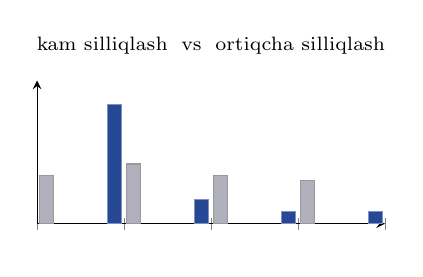
\begin{tikzpicture}
  \begin{axis}[ybar, bar width=5pt, width=6.0cm, height=3.4cm, ymin=0, ymax=0.6,
      symbolic x coords={a,b,c,d,e}, xtick=data, xticklabels={,,,,},
      ytick=\empty, axis y line=left, axis x line=bottom,
      title={\scriptsize kam silliqlash \;vs\; ortiqcha silliqlash}, title style={font=\scriptsize}]
    \addplot+[fill=seenc,draw=seenc!60] coordinates {(a,0.05)(b,0.5)(c,0.1)(d,0.05)(e,0.05)};
    \addplot+[fill=unseenc,draw=black!40] coordinates {(a,0.2)(b,0.25)(c,0.2)(d,0.18)(e,0.18)};
  \end{axis}
\end{tikzpicture}\\[-2pt]
{\scriptsize ko\uzq{}k: ishonchli \quad kulrang: tekis (foydasiz)}

\vspace{3pt}
\begin{tcolorbox}[okbox,left=2mm,right=2mm,top=1mm,bottom=1mm]
\scriptsize
Past perplexity --- \textbf{vosita}, maqsad emas. Yakuniy vazifa sifati
(to\uzq{}ldirish to\uzq{}g\uzq{}riligi) muhimroq. Yaxshiroq usullar: add-$k$
(kichikroq $+k$), \textit{backoff} (kam uchrasa qisqaroq N-gramga tushadi), Kneser--Ney.
\end{tcolorbox}
\end{column}
\end{columns}

\end{frame}

% ================================================================
\section[POS]{So\uzq{}z turkumlari va Markov zanjirlari}
% ================================================================

% ----------------------------------------------------------------
% [F3] INTUITSIYA: teglar
% ----------------------------------------------------------------
\begin{frame}{Intuitsiya: har so\uzq{}zga turkum, har turkum oldingisiga bog\uzq{}liq}
\footnotesize

\begin{columns}[T,totalwidth=\textwidth]
\begin{column}{0.52\textwidth}
So\uzq{}z turkumini aniqlash (\textit{Part-of-Speech, POS}): har so\uzq{}zga
\textbf{teg} --- ot (NN), fe\uzq{}l (VB), sifat\dots

\vspace{4pt}
\textbf{Markov g\uzq{}oyasi:} keyingi teg asosan \emph{oldingi} tegga bog\uzq{}liq.
Otdan keyin ko\uzq{}pincha fe\uzq{}l, sifatdan keyin ot\dots

\vspace{6pt}
\begin{tcolorbox}[okbox,left=2mm,right=2mm,top=1mm,bottom=1mm]
\scriptsize
Bir xil so\uzq{}z turli teg olishi mumkin: \textbf{kontekst} hal qiladi.
Markov zanjiri teglar orasidagi \textbf{o\uzq{}tishlar}ni modellaydi.
\end{tcolorbox}
\end{column}

\begin{column}{0.46\textwidth}
\centering
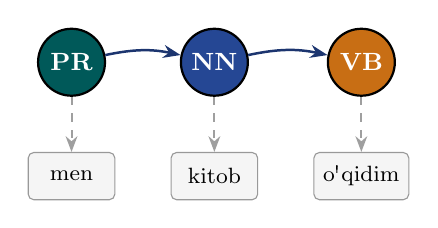
\begin{tikzpicture}[>=Stealth,node distance=6mm]
  \node[wbox] (w1) {men};
  \node[wbox,right=7mm of w1] (w2) {kitob};
  \node[wbox,right=7mm of w2] (w3) {o\uzq{}qidim};
  \node[state,fill=teal!70!black,text=white,above=7mm of w1] (t1) {PR};
  \node[nn,above=7mm of w2] (t2) {NN};
  \node[vb,above=7mm of w3] (t3) {VB};
  \draw[emit] (t1)--(w1); \draw[emit] (t2)--(w2); \draw[emit] (t3)--(w3);
  \draw[tran,bend left=12] (t1) to (t2);
  \draw[tran,bend left=12] (t2) to (t3);
\end{tikzpicture}\\[3pt]
{\scriptsize teglar (yuqorida) \textbf{zanjir} hosil qiladi;\\
so\uzq{}zlar (pastda) --- kuzatiladigan natija\\[2pt]
PR --- olmosh, NN --- ot, VB --- fe\uzq{}l}
\end{column}
\end{columns}

\end{frame}

% ----------------------------------------------------------------
% [G3] RASMIY TA'RIF: Markov zanjiri (state diagram)
% ----------------------------------------------------------------
\begin{frame}{Markov zanjiri: rasmiy ta\uzq{}rif}
\footnotesize

\begin{tcolorbox}[defbox,left=2mm,right=2mm,top=1mm,bottom=1mm]
\[
P(s_1 s_2 \dots s_T) \;=\; \pi(s_1)\prod_{t=2}^{T} A(s_t \mid s_{t-1})
\]
\end{tcolorbox}

\vspace{1pt}
$s_t$ --- $t$-holat (teg); $\pi(s_1)$ --- boshlang\uzq{}ich ehtimol;
$A(s_t\mid s_{t-1})$ --- o\uzq{}tish (\textit{transition}) ehtimoli. 1-tartibli zanjir:
keyingi holat faqat \emph{bitta} oldingisiga bog\uzq{}liq.
Har bir satr yig\uzq{}indisi $1$: $\sum_j A(j\mid i)=1$ (shartli taqsimot).

\vspace{3pt}
\begin{columns}[c,totalwidth=\textwidth]
\begin{column}{0.46\textwidth}
\centering
{\scriptsize O\uzq{}tish matritsasi $A$ (soddalashtirilgan o\uzq{}quv misoli):}\\[2pt]
\begin{tabular}{c|cc}
\toprule
 & $\to$ NN & $\to$ VB \\
\midrule
NN & 0.4 & 0.6 \\
VB & 0.3 & 0.7 \\
\bottomrule
\end{tabular}\\[5pt]
$\pi(\mathrm{NN})=0.7,\quad \pi(\mathrm{VB})=0.3$
\end{column}

\begin{column}{0.50\textwidth}
\centering
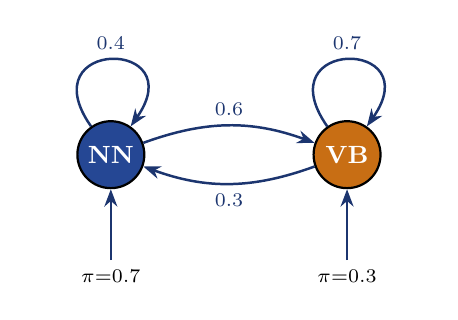
\begin{tikzpicture}[>=Stealth]
  \node[nn] (NN) at (0,0) {NN};
  \node[vb] (VB) at (3.0,0) {VB};
  \draw[tran,bend left=20] (NN) to node[above,font=\scriptsize]{0.6} (VB);
  \draw[tran,bend left=20] (VB) to node[below,font=\scriptsize]{0.3} (NN);
  \draw[tran] (NN) to[out=125,in=55,looseness=7] node[above,font=\scriptsize]{0.4} (NN);
  \draw[tran] (VB) to[out=125,in=55,looseness=7] node[above,font=\scriptsize]{0.7} (VB);
  \node[font=\scriptsize,below=9mm of NN] (pn) {$\pi{=}0.7$};
  \node[font=\scriptsize,below=9mm of VB] (pv) {$\pi{=}0.3$};
  \draw[tran] (pn)--(NN); \draw[tran] (pv)--(VB);
\end{tikzpicture}\\[1pt]
{\scriptsize o\uzq{}qlar --- o\uzq{}tish ehtimollari; pastdan --- $\pi$ (boshlanish)}
\end{column}
\end{columns}

\end{frame}

% ----------------------------------------------------------------
% [H3] KELTIRIB CHIQARISH: qo'shma ehtimol -> Markov  (statik)
% ----------------------------------------------------------------
\begin{frame}{Keltirib chiqarish: to\uzq{}liq qo\uzq{}shma ehtimoldan Markovgacha}
\footnotesize

\begin{columns}[T,totalwidth=\textwidth]
\begin{column}{0.62\textwidth}
\textbf{1-qadam.} Teglar ketma-ketligining to\uzq{}liq ehtimoli (zanjir qoidasi):
\[
P(s_1\dots s_T)=\pi(s_1)\prod_{t=2}^{T} P(s_t\mid s_1\dots s_{t-1})
\]

\textbf{2-qadam.} 1-tartibli Markov taxmini --- faqat oldingi holat muhim:
\[
P(s_t\mid s_1\dots s_{t-1}) \approx P(s_t\mid s_{t-1}) = A(s_t\mid s_{t-1})
\]

\textbf{3-qadam.} Demak:
\[
P(s_1\dots s_T)=\pi(s_1)\prod_{t=2}^{T} A(s_t\mid s_{t-1})
\]

\vspace{2pt}
Bu --- N-gram bilan bir xil g\uzq{}oya, faqat so\uzq{}zlar o\uzq{}rniga \textbf{teglar} ustida.
\end{column}

\begin{column}{0.36\textwidth}
\centering
{\scriptsize \textbf{faqat oxirgi teg muhim}}\\[3pt]
\resizebox{\linewidth}{!}{%
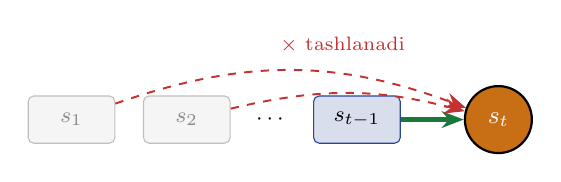
\begin{tikzpicture}[>=Stealth,node distance=3.5mm]
  \node[wbox,draw=black!25,text=black!45] (a) {$s_1$};
  \node[wbox,draw=black!25,text=black!45,right=of a] (b) {$s_2$};
  \node[font=\footnotesize,right=2mm of b] (d) {$\cdots$};
  \node[wbox,right=2mm of d,fill=NNc!18,draw=NNc] (c) {$s_{t-1}$};
  \node[state,fill=VBc,text=white,right=8mm of c] (st) {$s_t$};
  \draw[best] (c)--(st);
  \draw[dep,dashed,line width=0.7pt] (a) to[bend left=20] (st);
  \draw[dep,dashed,line width=0.7pt] (b) to[bend left=14] (st);
  \node[HiRed,font=\scriptsize] at ($(b)!0.5!(st)+(0,0.95)$) {$\times$ tashlanadi};
\end{tikzpicture}}\\[2pt]
{\scriptsize yashil --- saqlanadi;\\ qizil --- e\uzq{}tiborsiz qoldiriladi}
\end{column}
\end{columns}

\end{frame}

% ----------------------------------------------------------------
% [I3] QO'LDA MISOL: P(NN,VB)=0.42
% ----------------------------------------------------------------
\begin{frame}{Qo\uzq{}lda misol: teg ketma-ketligi ehtimoli}
\footnotesize

\begin{columns}[c,totalwidth=\textwidth]
\begin{column}{0.52\textwidth}
$\pi(\mathrm{NN})=0.7,\quad A(\mathrm{VB}\mid \mathrm{NN})=0.6$
\;\footnotesize(soddalashtirilgan o\uzq{}quv misoli).

\vspace{4pt}
Hisoblaymiz:
\begin{align*}
P(\mathrm{NN},\mathrm{VB}) &= \pi(\mathrm{NN})\cdot A(\mathrm{VB}\mid \mathrm{NN})\\
                           &= 0.7 \times 0.6 = \mathbf{0.42}
\end{align*}

\vspace{2pt}
Bu faqat \emph{teglar} ehtimoli (so\uzq{}zlarsiz). Keyingi tsiklda so\uzq{}zlar
(kuzatuvlar) qo\uzq{}shilib, HMM hosil bo\uzq{}ladi.
\end{column}

\begin{column}{0.46\textwidth}
\centering
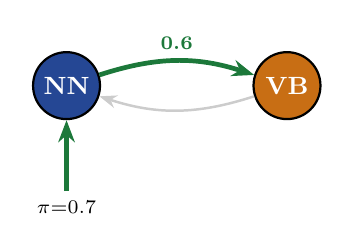
\begin{tikzpicture}[>=Stealth]
  \node[nn] (NN) at (0,0) {NN};
  \node[vb] (VB) at (2.8,0) {VB};
  \draw[best,bend left=18] (NN) to node[above,font=\scriptsize\bfseries]{0.6} (VB);
  \node[font=\scriptsize,below=9mm of NN] (pn) {$\pi{=}0.7$};
  \draw[best] (pn)--(NN);
  \draw[tran,gray!40,bend left=18] (VB) to (NN);
\end{tikzpicture}\\[4pt]
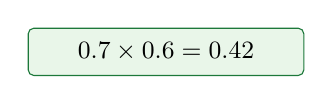
\begin{tikzpicture}
  \node[wbox,fill=greenbg,draw=ForestGreen,minimum width=3.5cm,font=\small]
    {$0.7 \times 0.6 = 0.42$};
\end{tikzpicture}\\[2pt]
{\scriptsize boshlash $\to$ NN, so\uzq{}ng NN $\to$ VB}
\end{column}
\end{columns}

\end{frame}

% ----------------------------------------------------------------
% [J3] SIZNING VAZIFANGIZ: P(VB,NN)=0.09   (2 betli overlay)
% ----------------------------------------------------------------
\begin{frame}{Sizning vazifangiz: teskari ketma-ketlik}
\small

\only<1>{
\begin{tcolorbox}[warnbox,title=Vazifa]
$\pi(\mathrm{VB})=0.3,\quad A(\mathrm{NN}\mid \mathrm{VB})=0.3$.
\[
P(\mathrm{VB},\mathrm{NN}) = ?
\]
\end{tcolorbox}
}

\only<2>{
\begin{columns}[c,totalwidth=\textwidth]
\begin{column}{0.54\textwidth}
\begin{tcolorbox}[warnbox,title=Vazifa]
$\pi(\mathrm{VB})=0.3,\ A(\mathrm{NN}\mid \mathrm{VB})=0.3;\quad
P(\mathrm{VB},\mathrm{NN})=\,?$
\end{tcolorbox}

\vspace{3pt}
\begin{tcolorbox}[okbox,title=Javob]
\begin{align*}
P(\mathrm{VB},\mathrm{NN}) &= \pi(\mathrm{VB})\cdot A(\mathrm{NN}\mid \mathrm{VB})\\
                           &= 0.3 \times 0.3 = 0.09
\end{align*}
\footnotesize
$0.09 < 0.42$ --- bu korpusda gap ot bilan boshlanib fe\uzq{}l bilan davom etishi
ancha ehtimoliyroq (NN$\to$VB).
\end{tcolorbox}
\end{column}

\begin{column}{0.44\textwidth}
\centering
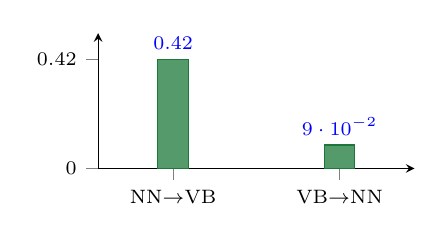
\begin{tikzpicture}
  \begin{axis}[probbars, bar shift=0pt, enlarge x limits=0.45, width=5.6cm, height=3.3cm, ymax=0.52,
      ytick={0,0.42},
      symbolic x coords={NN$\to$VB, VB$\to$NN}, xtick=data,
      x tick label style={font=\scriptsize}]
    \addplot+[fill=ForestGreen!75,draw=ForestGreen] coordinates {(NN$\to$VB,0.42) (VB$\to$NN,0.09)};
  \end{axis}
\end{tikzpicture}\\[1pt]
{\scriptsize $0.42$ --- ehtimoliyroq teg tartibi}
\end{column}
\end{columns}
}

\end{frame}

% ----------------------------------------------------------------
% [K3] KOD <-> FORMULA: Markov  [fragile]
% ----------------------------------------------------------------
\begin{frame}[fragile]{Kod va formula: Markov ketma-ketligi}
\scriptsize

\begin{columns}[T,totalwidth=\textwidth]
\begin{column}{0.60\textwidth}
\textbf{Python kodi}

\begin{tcolorbox}[defbox,left=2mm,right=2mm,top=1mm,bottom=1mm]
\begin{verbatim}
pi = {"NN": 0.7, "VB": 0.3}
A = {("NN","NN"): 0.4, ("NN","VB"): 0.6,
     ("VB","NN"): 0.3, ("VB","VB"): 0.7}

def seq_prob(tags):
    p = pi[tags[0]]
    for i in range(1, len(tags)):
        p *= A[(tags[i-1], tags[i])]
    return p

print(round(seq_prob(["NN","VB"]), 2))  # 0.42
print(round(seq_prob(["VB","NN"]), 2))  # 0.09
\end{verbatim}
\end{tcolorbox}
\end{column}

\begin{column}{0.38\textwidth}
\textbf{Kod va formula mosligi}

\begin{tabular}{@{}l l@{}}
\toprule
\textbf{Kod} & \textbf{Formula} \\
\midrule
\texttt{pi[tags[0]]}    & $\pi(s_1)$ \\
\texttt{A[(prev,cur)]}  & $A(s_t\mid s_{t-1})$ \\
\texttt{p *= ...}       & $\prod$ \\
\bottomrule
\end{tabular}

\vspace{6pt}
\begin{tcolorbox}[defbox,left=2mm,right=2mm,top=1mm,bottom=1mm]
\scriptsize
$A$ --- o\uzq{}tish matritsasi (lug\uzq{}at sifatida). 5-amaliyotdagi
\texttt{m05b POSTagger} moduli shuni kengaytiradi.
\end{tcolorbox}
\end{column}
\end{columns}

\end{frame}

% ----------------------------------------------------------------
% [L3] CHEKLOV: Markov tuzog'i
% ----------------------------------------------------------------
\begin{frame}{Markov tuzog\uzq{}i: uzoq bog\uzq{}liqlik ko\uzq{}rinmaydi}
\footnotesize

\begin{columns}[T,totalwidth=\textwidth]
\begin{column}{0.50\textwidth}
\begin{tcolorbox}[warnbox,title=1-tartib cheklovi,left=2mm,right=2mm,top=1mm,bottom=1mm]
Keyingi holat faqat \emph{bitta} oldingisiga bog\uzq{}liq. Lekin:

\vspace{3pt}
\centering\itshape ``agar yomg\uzq{}ir yog\uzq{}sa\dots\ biz uyda qolamiz''

\vspace{3pt}
\raggedright ``qolamiz'' so\uzq{}zi ``agar''ga bog\uzq{}liq --- ammo ular orasida
ko\uzq{}p so\uzq{}z bor. 1-tartibli Markov buni \textbf{ko\uzq{}rmaydi}.
\end{tcolorbox}
\end{column}

\begin{column}{0.48\textwidth}
\centering
\resizebox{\linewidth}{!}{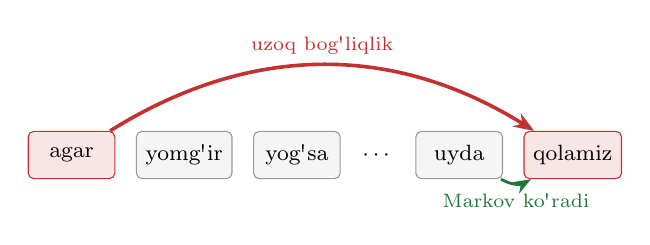
\begin{tikzpicture}[>=Stealth,node distance=2.6mm]
  \node[wbox,fill=HiRed!12,draw=HiRed] (a) {agar};
  \node[wbox,right=of a] (b) {yomg\uzq{}ir};
  \node[wbox,right=of b] (c) {yog\uzq{}sa};
  \node[font=\footnotesize,right=1.5mm of c] (d) {$\cdots$};
  \node[wbox,right=1.5mm of d] (e) {uyda};
  \node[wbox,fill=HiRed!12,draw=HiRed,right=of e] (f) {qolamiz};
  \draw[dep] (a) to[bend left=32] node[above,font=\scriptsize]{uzoq bog\uzq{}liqlik} (f);
  \draw[tran,ForestGreen,line width=1pt] (e) to[bend right=30] node[below,font=\scriptsize]{Markov ko\uzq{}radi} (f);
\end{tikzpicture}}\\[4pt]
{\scriptsize Yuqori tartib (2-, 3-) biroz yordam beradi.\\
To\uzq{}liq yechim: \textbf{LSTM} va \textbf{Transformer} (keyingi haftalarda).}
\end{column}
\end{columns}

\end{frame}

% ----------------------------------------------------------------
% [M3] O'ZBEK POS MUAMMOLARI
% ----------------------------------------------------------------
\begin{frame}{O\uzq{}zbek POS teglashda amaliy muammolar}
\footnotesize

\begin{columns}[T,totalwidth=\textwidth]
\begin{column}{0.52\textwidth}

O\uzq{}zbek tilida bitta so\uzq{}z shakli ko\uzq{}p grammatik ma\uzq{}lumot tashiydi:

\begin{itemize}\setlength\itemsep{3pt}
  \item \texttt{kitoblarimizdan}: ot $+$ ko\uzq{}plik $+$ egalik $+$ kelishik;
  \item \texttt{yozgan}: fe\uzq{}ldan yasalgan sifatdosh shakl; gapda sifatga
        yaqin vazifada kelishi mumkin;
  \item erkinroq so\uzq{}z tartibi teglar ketma-ketligini oldindan taxmin qilishni
        murakkablashtiradi.
\end{itemize}

\vspace{3pt}
\centering
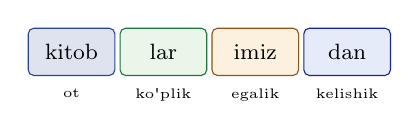
\begin{tikzpicture}[node distance=1.5pt,>=Stealth]
  \node[wbox,fill=NNc!15,draw=NNc] (m1) {kitob};
  \node[wbox,fill=greenbg,draw=ForestGreen,right=of m1] (m2) {lar};
  \node[wbox,fill=creambg,draw=brownbar,right=of m2] (m3) {imiz};
  \node[wbox,fill=bluebg,draw=mainblue,right=of m3] (m4) {dan};

  \node[font=\tiny,below=1pt of m1] {ot};
  \node[font=\tiny,below=1pt of m2] {ko\uzq{}plik};
  \node[font=\tiny,below=1pt of m3] {egalik};
  \node[font=\tiny,below=1pt of m4] {kelishik};
\end{tikzpicture}

\vspace{2pt}
{\scriptsize bitta so\uzq{}z --- to\uzq{}rt morfema}

\end{column}

\begin{column}{0.46\textwidth}

\begin{tcolorbox}[okbox,title=Amaliy yechimlar,
left=2mm,right=2mm,top=1mm,bottom=1mm]
\footnotesize
HMM uchun \textbf{teglangan korpus} zarur. Korpus kichik bo\uzq{}lsa:

\begin{itemize}\setlength\itemsep{3pt}
  \item morfologik analizator orqali mumkin bo\uzq{}lgan teglar toraytiriladi;
  \item qoida va lug\uzq{}atlar bilan xatolar kamaytiriladi;
  \item qo\uzq{}lda tekshirilgan namunalar bilan model baholanadi;
  \item keyinroq neyron modellar bilan gibrid yondashuv quriladi.
\end{itemize}
\end{tcolorbox}

\end{column}
\end{columns}

\end{frame}

% ================================================================
\section[HMM]{Yashirin Markov modeli va Viterbi}
% ================================================================

% ----------------------------------------------------------------
% [F4] INTUITSIYA: teglar yashirin
% ----------------------------------------------------------------
\begin{frame}{Intuitsiya: teglar yashirin, so\uzq{}zlar ko\uzq{}rinadi}
\footnotesize

\begin{columns}[T,totalwidth=\textwidth]
\begin{column}{0.52\textwidth}
\textbf{Markov zanjiri} (3-bo\uzq{}lim): teglar \textbf{ko\uzq{}rinadi}.\quad
\textbf{HMM}: teglar \textbf{yashirin} --- faqat so\uzq{}zlar ko\uzq{}rinadi.

\vspace{2pt}
Biz \textbf{so\uzq{}zlar}ni ko\uzq{}ramiz (\texttt{nlp}, \texttt{yozdi}), lekin
\textbf{teglar} (NN, VB) yashirin. Yashirin Markov modeli (HMM):
\begin{itemize}\setlength\itemsep{2pt}
  \item teglar Markov zanjiri bo\uzq{}ylab o\uzq{}tadi ($A$ --- o\uzq{}tish);
  \item har teg so\uzq{}zni ``chiqaradi'' ($B$ --- chiqarish, \textit{emission}).
\end{itemize}

\vspace{1pt}
{\scriptsize $\pi,A,B$ --- chastotadan (MLE) o\uzq{}rganiladi (teglangan korpusdan).}

\vspace{2pt}
\textbf{Vazifa:} so\uzq{}zlar berilgan, eng ehtimoliy teg ketma-ketligini topish.

\vspace{4pt}
\begin{tcolorbox}[okbox,left=2mm,right=2mm,top=1mm,bottom=1mm]
\scriptsize
Barcha teg yo\uzq{}llarini sinash eksponensial ($S^{T}$).
\textbf{Viterbi} --- DP bilan eng yaxshi yo\uzq{}lni $O(T\cdot S^{2})$ da topadi.
\end{tcolorbox}
\end{column}

\begin{column}{0.46\textwidth}
\centering
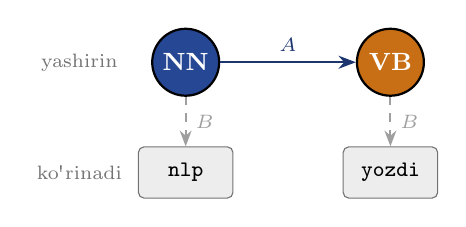
\begin{tikzpicture}[>=Stealth]
  \node[font=\scriptsize,text=black!55] at (-1.35,1.4) {yashirin};
  \node[font=\scriptsize,text=black!55] at (-1.35,0)   {ko\uzq{}rinadi};
  \node[nn] (NN) at (0,1.4) {NN};
  \node[vb] (VB) at (2.6,1.4) {VB};
  \draw[tran] (NN) to node[above,font=\scriptsize]{$A$} (VB);
  \node[obs] (o1) at (0,0) {nlp};
  \node[obs] (o2) at (2.6,0) {yozdi};
  \draw[emit] (NN)-- node[right,font=\scriptsize]{$B$} (o1);
  \draw[emit] (VB)-- node[right,font=\scriptsize]{$B$} (o2);
\end{tikzpicture}\\[4pt]
{\scriptsize teglar zanjiri ($A$) so\uzq{}zlarni chiqaradi ($B$)}
\end{column}
\end{columns}

\end{frame}

% ----------------------------------------------------------------
% [G4] RASMIY TA'RIF: HMM + Viterbi
% ----------------------------------------------------------------
\begin{frame}{HMM va Viterbi: asosiy g\uzq{}oya}
\footnotesize

\textbf{HMM} (\textit{Hidden Markov Model} — yashirin Markov modeli)
ko\uzq{}rinadigan so\uzq{}zlar ortida yashirin POS teglar ketma-ketligi bor deb qaraydi.

\vspace{3pt}

\begin{columns}[T,totalwidth=\textwidth]
%------------------------------------------------
\begin{column}{0.49\textwidth}

\textbf{Model qismlari}

\begin{itemize}\setlength\itemsep{3pt}
  \item $\pi(j)$ — gap boshida $j$ teg kelish ehtimoli;
  \item $A(j\mid i)$ — $i$ tegdan $j$ tegga o\uzq{}tish ehtimoli;
  \item $B(o_t\mid j)$ — $j$ tegda $o_t$ so\uzq{}zini ko\uzq{}rish ehtimoli.
\end{itemize}

\vspace{4pt}

\begin{tcolorbox}[defbox,left=2mm,right=2mm,top=1mm,bottom=1mm]
\scriptsize
\textbf{Viterbi} — barcha teg ketma-ketliklarini sinamay,
dinamik dasturlash orqali eng ehtimoliy yo\uzq{}lni topadi.
\end{tcolorbox}

\vspace{3pt}

\textbf{Asosiy rekurrensiya}
\[
\delta_t(j)=
\Big[\max_i \delta_{t-1}(i)A(j\mid i)\Big]B(o_t\mid j)
\]

\end{column}

%------------------------------------------------
\begin{column}{0.47\textwidth}

\textbf{Formula talqini}

\begin{itemize}\setlength\itemsep{3pt}
  \item $\delta_t(j)$ — $t$-pozitsiyada $j$ teg bilan tugaydigan eng yaxshi yo\uzq{}l balli;
  \item $\max_i$ — oldingi teglardan eng yaxshisini tanlash;
  \item $B(o_t\mid j)$ — hozirgi so\uzq{}zning $j$ tegga mosligi.
\end{itemize}

\vspace{2pt}

\centering
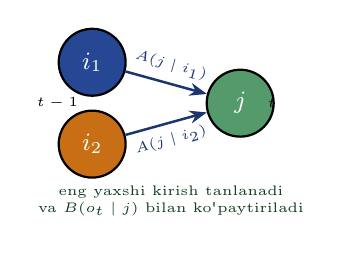
\begin{tikzpicture}[scale=0.80,>=Stealth,every node/.style={font=\scriptsize}]
  \node[nn] (a) at (0,0.75) {$i_1$};
  \node[vb] (b) at (0,-0.55) {$i_2$};
  \node[state,fill=ForestGreen!75,text=white] (t) at (2.35,0.10) {$j$};

  \draw[tran] (a) -- node[above,sloped,font=\tiny] {$A(j\mid i_1)$} (t);
  \draw[tran] (b) -- node[below,sloped,font=\tiny] {$A(j\mid i_2)$} (t);

  \node[font=\tiny] at (-0.55,0.10) {$t-1$};
  \node[font=\tiny] at (2.85,0.10) {$t$};

  \node[align=center,font=\tiny,text=ForestGreen!50!black] at (1.25,-1.45)
  {eng yaxshi kirish tanlanadi\\
  va $B(o_t\mid j)$ bilan ko\uzq{}paytiriladi};
\end{tikzpicture}

\end{column}
\end{columns}

\end{frame}
% ----------------------------------------------------------------
% [H4] KELTIRIB CHIQARISH: nega Viterbi DP  (statik)
% ----------------------------------------------------------------
\begin{frame}{Keltirib chiqarish: nega Viterbi DP ishlaydi?}
\footnotesize

\begin{columns}[T,totalwidth=\textwidth]
\begin{column}{0.62\textwidth}
\textbf{1-qadam.} Maqsad --- $\arg\max_{s} P(s\mid o)$; ammo $o$ (so\uzq{}zlar)
berilganda $P(o)$ $s$ ga bog\uzq{}liq emas, shuning uchun qo\uzq{}shma ehtimolni
maksimallashtiramiz:
$\displaystyle \arg\max_{s_1\dots s_T} P(s_1\dots s_T,\, o_1\dots o_T)$.
Barcha yo\uzq{}llar --- $S^{T}$ ta (juda ko\uzq{}p).

\vspace{3pt}
\textbf{2-qadam.} Kuzatuv: $t$ da $j$ holatda tugaydigan eng yaxshi yo\uzq{}l faqat
$t{-}1$ dagi eng yaxshi yo\uzq{}llarga tayanadi (Markov xossasi).

\vspace{3pt}
\textbf{3-qadam.} Shuning uchun har qadamda har holat uchun eng yaxshi kirishni saqlaymiz:
\[
\delta_t(j)=\Big[\max_{i}\delta_{t-1}(i)A(j\mid i)\Big]B(o_t\mid j)
\]

\vspace{2pt}
Eksponensial qidiruv $O(TS^{2})$ ga tushadi --- 4-ma\uzq{}ruzadagi
\texttt{edit\_distance} bilan bir xil DP mantiqi.
\end{column}

\begin{column}{0.36\textwidth}
\centering
{\scriptsize \textbf{$S^{T}$ yo\uzq{}l $\Rightarrow$ qadamli max}}\\[3pt]
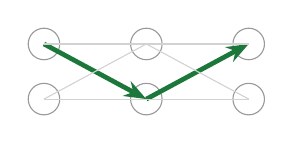
\begin{tikzpicture}[>=Stealth,every node/.style={font=\tiny}]
  \foreach \x in {0,1.3,2.6}{
    \node[circle,draw=black!40,minimum size=4mm,inner sep=0] at (\x,0.7){};
    \node[circle,draw=black!40,minimum size=4mm,inner sep=0] at (\x,0){};
  }
  \draw[best] (0,0.7)--(1.3,0); \draw[best] (1.3,0)--(2.6,0.7);
  \draw[gray!35] (0,0)--(1.3,0); \draw[gray!35] (0,0.7)--(1.3,0.7);
  \draw[gray!35] (1.3,0.7)--(2.6,0.7); \draw[gray!35] (1.3,0)--(2.6,0);
  \draw[gray!35] (0,0)--(1.3,0.7); \draw[gray!35] (1.3,0.7)--(2.6,0);
\end{tikzpicture}\\[2pt]
{\scriptsize Viterbi \textbf{panjarasi} (\textit{trellis}); yashil --- saqlangan
eng yaxshi yo\uzq{}l}
\end{column}
\end{columns}

\end{frame}

% ----------------------------------------------------------------
% [I4] QO'LDA HISOB: Viterbi trellis  --- MARKAZIY SLAYD
% ----------------------------------------------------------------
\begin{frame}{Qo\uzq{}lda hisob: Viterbi --- $\delta(\mathrm{VB},t{=}2)=0.3402$}
\scriptsize
\textbf{Parametrlar} (soddalashtirilgan o\uzq{}quv misoli):\;
$\pi(\mathrm{NN}){=}0.7,\ \pi(\mathrm{VB}){=}0.3$;\quad
$B(\text{nlp}|\mathrm{NN}){=}0.9,\ B(\text{nlp}|\mathrm{VB}){=}0.1,\
 B(\text{yozdi}|\mathrm{NN}){=}0.1,\ B(\text{yozdi}|\mathrm{VB}){=}0.9$;\quad
$A(\mathrm{VB}|\mathrm{NN}){=}0.6,\ A(\mathrm{NN}|\mathrm{VB}){=}0.3,\
 A(\mathrm{NN}|\mathrm{NN}){=}0.4,\ A(\mathrm{VB}|\mathrm{VB}){=}0.7$

\vspace{3pt}
\begin{columns}[T,totalwidth=\textwidth]
\begin{column}{0.40\textwidth}
{\small \textbf{$t{=}1$ (nlp):}}
\begin{align*}
\delta_1(\mathrm{NN}) &= 0.7\cdot 0.9 = 0.63\\
\delta_1(\mathrm{VB}) &= 0.3\cdot 0.1 = 0.03
\end{align*}
{\small \textbf{$t{=}2$ (yozdi), VB:}}
\begin{align*}
\delta_2(\mathrm{VB}) &= \max(0.63\cdot 0.6,\ 0.03\cdot 0.7)\cdot 0.9\\
                      &= 0.378\cdot 0.9 = \mathbf{0.3402}
\end{align*}
\begin{tcolorbox}[defbox,left=2mm,right=2mm,top=1mm,bottom=1mm]
\scriptsize
Ertangi 5-amaliyotning birinchi assert\uzq{}i:\\
\texttt{abs(delta\_VB\_t2 - 0.3402) < 1e-4}
\end{tcolorbox}
\end{column}

\begin{column}{0.58\textwidth}
\centering
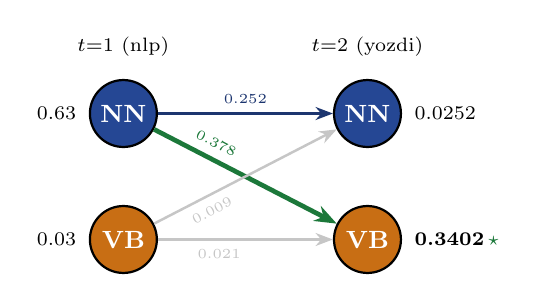
\begin{tikzpicture}[>=Stealth,every node/.style={font=\scriptsize}]
  \node at (0,2.05) {$t{=}1$ \scriptsize(nlp)};
  \node at (3.1,2.05) {$t{=}2$ \scriptsize(yozdi)};
  \node[nn] (n1) at (0,1.2)  {NN};  \node[left=1pt of n1] {0.63};
  \node[vb] (v1) at (0,-0.4) {VB};  \node[left=1pt of v1] {0.03};
  \node[nn] (n2) at (3.1,1.2)  {NN};  \node[right=1pt of n2] {0.0252};
  \node[vb] (v2) at (3.1,-0.4) {VB};  \node[right=1pt of v2] {\textbf{0.3402}\,{\color{ForestGreen}$\star$}};
  \draw[best] (n1) to node[sloped,above,font=\tiny,pos=0.30]{0.378} (v2);
  \draw[tran] (n1) -- node[above,font=\tiny]{0.252} (n2);
  \draw[tran,gray!45] (v1) -- node[below,font=\tiny,pos=0.35]{0.021} (v2);
  \draw[tran,gray!45] (v1) to node[sloped,below,font=\tiny,pos=0.28]{0.009} (n2);
\end{tikzpicture}\\[2pt]
{\scriptsize \textcolor{ForestGreen}{\textbf{yashil}} --- eng ehtimoliy yo\uzq{}l;
orqaga kuzatish: VB $\leftarrow$ NN $\Rightarrow$ \textbf{[NN, VB]}}
\end{column}
\end{columns}

\end{frame}

% ----------------------------------------------------------------
% [J4] SIZNING VAZIFANGIZ: delta2(NN)=0.0252  (2 betli overlay)
% ----------------------------------------------------------------
\begin{frame}{Sizning vazifangiz: $\delta_2(\mathrm{NN})$ ni hisoblang}
\small

\only<1>{
\begin{tcolorbox}[warnbox,title=Vazifa]
Xuddi shu HMM uchun $t=2$ (\textit{yozdi}) da NN qiymatini hisoblang.

\vspace{3pt}

\[
\delta_2(\mathrm{NN})
=
\max
\begin{cases}
\delta_1(\mathrm{NN})A(\mathrm{NN}\mid\mathrm{NN}),\\
\delta_1(\mathrm{VB})A(\mathrm{NN}\mid\mathrm{VB})
\end{cases}
\cdot B(\text{yozdi}\mid\mathrm{NN})
\]

\vspace{3pt}

\[
\delta_1(\mathrm{NN})=0.63,\quad
\delta_1(\mathrm{VB})=0.03
\]
\[
A(\mathrm{NN}\mid\mathrm{NN})=0.4,\quad
A(\mathrm{NN}\mid\mathrm{VB})=0.3,\quad
B(\text{yozdi}\mid\mathrm{NN})=0.1
\]
\end{tcolorbox}
}

\only<2>{
\begin{columns}[T,totalwidth=\textwidth]
%------------------------------------------------
\begin{column}{0.56\textwidth}

\begin{tcolorbox}[warnbox,title=Vazifa,left=2mm,right=2mm,top=1mm,bottom=1mm]
\[
\delta_2(\mathrm{NN})=?
\]
\end{tcolorbox}

\vspace{2pt}

\textbf{1-qadam. NN ga keladigan ikki yo\uzq{}lni hisoblaymiz}

\[
\mathrm{NN}\rightarrow\mathrm{NN}:\quad 0.63\cdot0.4=0.252
\]

\[
\mathrm{VB}\rightarrow\mathrm{NN}:\quad 0.03\cdot0.3=0.009
\]

\vspace{2pt}

\textbf{2-qadam. Eng katta kirishni tanlaymiz}

\[
\max(0.252,\;0.009)=0.252
\]

\vspace{2pt}

\textbf{3-qadam. \textit{yozdi} ning NN bo\uzq{}yicha ehtimoliga ko\uzq{}paytiramiz}

\[
\delta_2(\mathrm{NN})=0.252\cdot0.1=0.0252
\]

\end{column}

%------------------------------------------------
\begin{column}{0.40\textwidth}
\centering

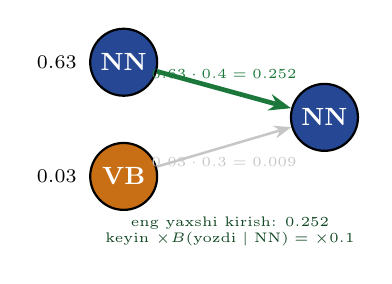
\begin{tikzpicture}[>=Stealth,every node/.style={font=\scriptsize}]
  \node[nn] (n1) at (0,1.0) {NN};
  \node[left=1pt of n1] {$0.63$};

  \node[vb] (v1) at (0,-0.45) {VB};
  \node[left=1pt of v1] {$0.03$};

  \node[nn] (n2) at (2.55,0.30) {NN};

  \draw[best] (n1) -- node[above,font=\tiny] {$0.63\cdot0.4=0.252$} (n2);
  \draw[tran,gray!45] (v1) -- node[below,font=\tiny] {$0.03\cdot0.3=0.009$} (n2);

  \node[font=\tiny,align=center,text=ForestGreen!60!black] at (1.35,-1.15)
  {eng yaxshi kirish: $0.252$\\
   keyin $\times B(\text{yozdi}\mid\mathrm{NN})=\times0.1$};
\end{tikzpicture}

\vspace{4pt}

\begin{tcolorbox}[okbox,left=2mm,right=2mm,top=1mm,bottom=1mm]
\scriptsize
\[
\boxed{\delta_2(\mathrm{NN})=0.0252}
\]

Bu faqat $t=2$ dagi \textbf{NN} katagi uchun hisob.
\end{tcolorbox}

\scriptsize
Oldingi hisobda $\delta_2(\mathrm{VB})=0.3402$ bo\uzq{}lsa,
$0.3402>0.0252$, demak $t=2$ da VB kuchliroq.

\end{column}
\end{columns}
}

\end{frame}

% ----------------------------------------------------------------
% [K4] KOD <-> FORMULA: Viterbi  [fragile]
% ----------------------------------------------------------------
\begin{frame}[fragile]{Kod va formula: Viterbi}
\scriptsize

\begin{columns}[T,totalwidth=\textwidth]
\begin{column}{0.64\textwidth}
\textbf{Python kodi}

\begin{tcolorbox}[defbox,left=2mm,right=2mm,top=1mm,bottom=1mm]
\begin{verbatim}
def viterbi(obs, states, pi, A, B):
    delta = [{s: pi[s]*B[(obs[0],s)] for s in states}]
    back = [{}]
    for t in range(1, len(obs)):
        d, bk = {}, {}
        for j in states:
            i = max(states,
                    key=lambda i: delta[t-1][i]*A[(i,j)])
            d[j] = delta[t-1][i]*A[(i,j)]*B[(obs[t],j)]
            bk[j] = i
        delta.append(d); back.append(bk)
    last = max(states, key=lambda s: delta[-1][s])
    path = [last]
    for t in range(len(obs)-1, 0, -1):
        last = back[t][last]; path.insert(0, last)
    return path, delta
\end{verbatim}
\end{tcolorbox}
\end{column}

\begin{column}{0.34\textwidth}
\textbf{Kod va formula mosligi}

\begin{tabular}{@{}l l@{}}
\toprule
\textbf{Kod} & \textbf{Formula} \\
\midrule
\texttt{pi[s]*B}    & $\delta_1(j)$ \\
\texttt{max(...A)}  & $\max_i \delta A$ \\
\texttt{*B[(o,j)]}  & $\cdot B(o_t\mid j)$ \\
\texttt{bk[j]=i}    & $\psi_t(j)$ \\
\bottomrule
\end{tabular}

\vspace{5pt}
\begin{tcolorbox}[defbox,left=2mm,right=2mm,top=1mm,bottom=1mm]
\scriptsize
\texttt{path == ["NN","VB"]};\\
\texttt{delta[1]["VB"]} $\approx$ \texttt{0.3402}.\\
5-amaliyotdagi \texttt{m05b POSTagger} shuni amalga oshiradi.
\end{tcolorbox}
\end{column}
\end{columns}

\end{frame}

% ----------------------------------------------------------------
% [L4] CHEKLOV: Viterbi underflow
% ----------------------------------------------------------------
\begin{frame}{Viterbi tuzog\uzq{}i: ehtimollar ko\uzq{}paytmasi kichrayadi}
\footnotesize

\begin{columns}[T,totalwidth=\textwidth]
%------------------------------------------------
\begin{column}{0.46\textwidth}

\begin{tcolorbox}[warnbox,title=Muammo: underflow,
left=2mm,right=2mm,top=1mm,bottom=1mm]
\scriptsize
Uzun ketma-ketlikda kichik ehtimollar ketma-ket ko\uzq{}paytiriladi:

\[
0.6^{50}\approx 8.1\cdot 10^{-12}
\]

Son juda kichrayganda kompyuter uni \textbf{0} deb saqlashi mumkin.
\end{tcolorbox}

\vspace{4pt}

\begin{tcolorbox}[okbox,title=Yechim: log fazo,
left=2mm,right=2mm,top=1mm,bottom=1mm]
\scriptsize
Ko\uzq{}paytma logarifmlar yig\uzq{}indisiga aylantiriladi:
\[
\log(ab)=\log a+\log b
\]

Viterbi amalda ko\uzq{}pincha \textbf{log-ehtimollar} bilan hisoblanadi.
\end{tcolorbox}

\end{column}

%------------------------------------------------
\begin{column}{0.50\textwidth}
\centering

\textbf{\scriptsize Ko\uzq{}paytma va log-ko\uzq{}paytma farqi}

\vspace{1pt}

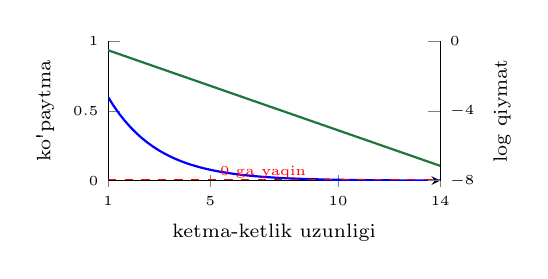
\begin{tikzpicture}
  \begin{axis}[
      width=5.8cm,
      height=3.35cm,
      xmin=1, xmax=14,
      ymin=0, ymax=1,
      xlabel={\scriptsize ketma-ketlik uzunligi},
      ylabel={\scriptsize ko\uzq{}paytma},
      axis y line*=left,
      axis x line=bottom,
      ytick={0,0.5,1},
      xtick={1,5,10,14},
      ticklabel style={font=\tiny},
      label style={font=\scriptsize}
    ]
    \addplot[blue,thick,domain=1:14,samples=60] {0.6^x};
    \addplot[red,dashed,domain=1:14,samples=2] {0.01};
    \node[red,font=\tiny,anchor=west] at (axis cs:5,0.06) {0 ga yaqin};
  \end{axis}

  \begin{axis}[
      width=5.8cm,
      height=3.35cm,
      xmin=1, xmax=14,
      ymin=-8, ymax=0,
      axis y line*=right,
      axis x line=none,
      ylabel={\scriptsize log qiymat},
      ytick={-8,-4,0},
      ticklabel style={font=\tiny},
      label style={font=\scriptsize}
    ]
    \addplot[ForestGreen,thick,domain=1:14,samples=60] {x*ln(0.6)};
  \end{axis}
\end{tikzpicture}

\vspace{2pt}

\begin{tcolorbox}[defbox,left=2mm,right=2mm,top=1mm,bottom=1mm]
\scriptsize
\textcolor{blue}{Ko\uzq{}paytma} tez 0 ga yaqinlashadi; 
\textcolor{ForestGreen}{log qiymat} esa tekis kamayadi va hisoblash uchun qulay.
\end{tcolorbox}

\end{column}
\end{columns}

\end{frame}

% ================================================================
\section[Xulosa]{Xulosa va amaliyotga ko\uzq{}prik}
% ================================================================

% ----------------------------------------------------------------
% [M] O'ZBEK TILIGA XOSLIK: SOV va agglutinatsiya
% ----------------------------------------------------------------
\begin{frame}{O\uzq{}zbek tilida: SOV tartibi va agglutinatsiya N-gramni qiynaydi}
\footnotesize

\begin{columns}[T,totalwidth=\textwidth]
\begin{column}{0.50\textwidth}
\textbf{1. SOV tartibi} (ega--to\uzq{}ldiruvchi--kesim, \textit{Subject--Object--Verb};
kesim oxirida):

\vspace{2pt}
\centering
\resizebox{\linewidth}{!}{%
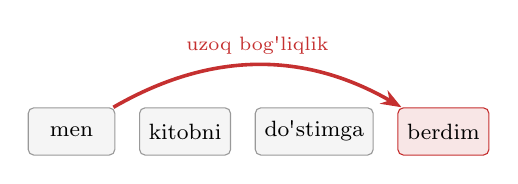
\begin{tikzpicture}[>=Stealth,node distance=3mm]
  \node[wbox] (a) {men};
  \node[wbox,right=of a] (b) {kitobni};
  \node[wbox,right=of b] (c) {do\uzq{}stimga};
  \node[wbox,fill=HiRed!12,draw=HiRed,right=of c] (d) {berdim};
  \draw[dep] (a) to[bend left=30] node[above,font=\scriptsize]{uzoq bog\uzq{}liqlik} (d);
\end{tikzpicture}}\\[2pt]
\raggedright
{\scriptsize Kesim (\texttt{berdim}) oxirida. Bigram ``men'' keyingisini taxmin
qiladi, lekin ma\uzq{}noni belgilovchi fe\uzq{}l \textbf{uzoqda} $\Rightarrow$ uzoq bog\uzq{}liqlik.}
\end{column}

\begin{column}{0.48\textwidth}
\textbf{2. Agglutinatsiya} (\textit{agglutination} --- qo\uzq{}shimchalar ketma-ket ulanishi):

\vspace{2pt}
\centering
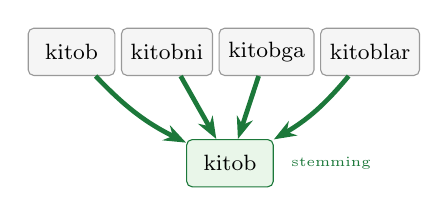
\begin{tikzpicture}[>=Stealth,node distance=2pt,every node/.style={font=\scriptsize}]
  \node[wbox] (w1) {kitob};
  \node[wbox,right=of w1] (w2) {kitobni};
  \node[wbox,right=of w2] (w3) {kitobga};
  \node[wbox,right=of w3] (w4) {kitoblar};
  \node[wbox,fill=greenbg,draw=ForestGreen,below=8mm of w2,xshift=8mm] (stem) {kitob};
  \draw[best] (w1) to[bend right=10] (stem);
  \draw[best] (w2) to (stem);
  \draw[best] (w3) to (stem);
  \draw[best] (w4) to[bend left=10] (stem);
  \node[font=\tiny,ForestGreen,right=1mm of stem] {stemming};
\end{tikzpicture}\\[2pt]
\begin{tcolorbox}[okbox,left=2mm,right=2mm,top=1mm,bottom=1mm]
\scriptsize
\textbf{Oqibat:} $|V|$ portlaydi; ko\uzq{}p N-gramlar 0/1 marta uchraydi
$\Rightarrow$ \textbf{siyrak} ma\uzq{}lumot, silliqlash ayniqsa muhim.
\textbf{Yechim:} stemming (\textit{stemming} --- so\uzq{}zni o\uzq{}zagiga keltirish) N-gramdan oldin $|V|$ ni kichraytiradi.
\end{tcolorbox}
\end{column}
\end{columns}

\end{frame}

% ----------------------------------------------------------------
% [N] SINTEZ: kontekst vs ma'lumot
% ----------------------------------------------------------------
\begin{frame}{Sintez: kontekst oshsa, ma\uzq{}lumot talabi ham oshadi}
\footnotesize

\begin{columns}[c,totalwidth=\textwidth]
\begin{column}{0.56\textwidth}
\renewcommand{\arraystretch}{1.18}
\begin{tabular}{@{}lll@{}}
\toprule
\textbf{Model} & \textbf{Kontekst} & \textbf{Murosa} \\
\midrule
Unigram & yo\uzq{}q & sodda, lekin kontekst yo\uzq{}q \\
Bigram & 1 oldingi & amaliy muvozanat \\
Trigram & 2 oldingi & aniqroq, ammo siyrakroq \\
HMM & yashirin teglar & ketma-ketlik teglash \\
\bottomrule
\end{tabular}

\vspace{5pt}

\begin{tcolorbox}[okbox,title=Asosiy g\uzq{}oya,
left=2mm,right=2mm,top=1mm,bottom=1mm]
\scriptsize
Asosiy mexanizm: \textbf{ehtimollikni sanash} $+$
\textbf{Markov taxmini} $+$ kerakli joyda \textbf{silliqlash}.
Viterbi shu g\uzq{}oyani POS teglar ketma-ketligini topishga qo\uzq{}llaydi.
\end{tcolorbox}
\end{column}

\begin{column}{0.42\textwidth}
\centering

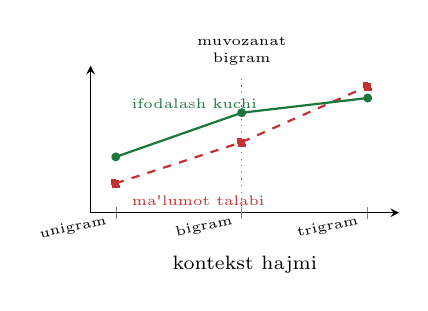
\begin{tikzpicture}[>=Stealth]
  \begin{axis}[
      width=5.5cm,
      height=3.45cm,
      xmin=0.8,xmax=3.25,
      ymin=0,ymax=1,
      axis y line=left,
      axis x line=bottom,
      xtick={1,2,3},
      xticklabels={unigram,bigram,trigram},
      x tick label style={font=\tiny,rotate=12,anchor=east},
      ytick=\empty,
      xlabel={\scriptsize kontekst hajmi},
      xlabel style={yshift=2pt},
      clip=false
    ]
    % data need / sparsity
    \addplot[HiRed,thick,dashed,mark=square*,mark size=1.2pt]
      coordinates {(1,0.20)(2,0.48)(3,0.86)};

    % possible accuracy / expressiveness
    \addplot[ForestGreen,thick,mark=*,mark size=1.2pt]
      coordinates {(1,0.38)(2,0.68)(3,0.78)};

    % bigram balance marker
    \draw[dotted,black!55] (axis cs:2,0) -- (axis cs:2,0.93);
    \node[font=\tiny,anchor=south,align=center] at (axis cs:2,0.94)
      {muvozanat\\bigram};

    % labels away from lines
    \node[font=\tiny,ForestGreen,anchor=west] at (axis cs:1.05,0.74)
      {ifodalash kuchi};
    \node[font=\tiny,HiRed,anchor=west] at (axis cs:1.05,0.08)
      {ma\uzq{}lumot talabi};
  \end{axis}
\end{tikzpicture}

\vspace{2pt}

{\scriptsize
Kontekst ko\uzq{}paysa, model kuchliroq bo\uzq{}lishi mumkin,
lekin uni ishonchli o\uzq{}qitish uchun ko\uzq{}proq ma\uzq{}lumot kerak.
}

\end{column}
\end{columns}

\end{frame}

% ----------------------------------------------------------------
% [O] SEMINAL MANBA: Rabiner (1989)
% ----------------------------------------------------------------
\begin{frame}{Seminal manba: Rabiner (1989)}
\footnotesize

\begin{tcolorbox}[defbox,left=2mm,right=2mm,top=1mm,bottom=1mm]
\small
Rabiner, L.R. (1989). \textbf{A Tutorial on Hidden Markov Models and Selected
Applications in Speech Recognition.} \textit{Proceedings of the IEEE}, 77(2), 257--286.
\end{tcolorbox}

\vspace{3pt}
\begin{columns}[T,totalwidth=\textwidth]
\begin{column}{0.54\textwidth}
\textbf{Ahamiyati}
\begin{itemize}\setlength\itemsep{2pt}
  \item HMM uchun klassik va keng qo\uzq{}llanadigan qo\uzq{}llanma.
  \item Uch masala: baholash (Forward), dekodlash (Viterbi),
        o\uzq{}rganish (Baum--Welch).
  \item Nutq, POS, bioinformatika --- hammasi shu doirada.
\end{itemize}

\vspace{2pt}
\centering
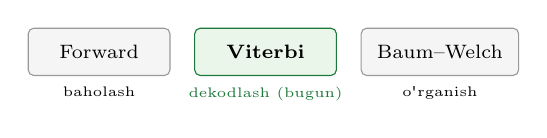
\begin{tikzpicture}[node distance=3mm]
  \node[wbox,minimum width=18mm] (f) {\scriptsize Forward};
  \node[wbox,minimum width=18mm,fill=greenbg,draw=ForestGreen,right=of f] (v) {\scriptsize\textbf{Viterbi}};
  \node[wbox,minimum width=20mm,right=of v] (bw) {\scriptsize Baum--Welch};
  \node[font=\tiny,below=0.5pt of f]{baholash};
  \node[font=\tiny,below=0.5pt of v,text=ForestGreen]{dekodlash (bugun)};
  \node[font=\tiny,below=0.5pt of bw]{o\uzq{}rganish};
\end{tikzpicture}
\end{column}

\begin{column}{0.44\textwidth}
\begin{tcolorbox}[warnbox,title=Muhokama savoli (5-amaliyotgacha o\uzq{}ylang),left=2mm,right=2mm,top=1mm,bottom=1mm]
HMM teglash uchun \textbf{teglangan korpus} kerak. O\uzq{}zbek tili uchun bunday
korpus kam. Bu cheklovni qanday yengish mumkin? (Maslahat: 4-hafta, BERT.)
\end{tcolorbox}
\end{column}
\end{columns}

\end{frame}

% ----------------------------------------------------------------
% [P] MAQSADLAR BAJARILDI
% ----------------------------------------------------------------
\begin{frame}{Bugungi maqsadlar bajarildi}
\footnotesize

\vspace{2pt}
\begin{enumerate}\setlength{\itemsep}{8pt}
  \item \gcheck\ \textbf{Keltirib chiqardik:} bigram MLE ---
    \colorbox{greenbg}{$P(\text{kitob}\mid\text{men})=2/3$} (zanjir qoidasi $+$ Markov taxmini).
  \item \gcheck\ \textbf{Hisobladik:} add-1 silliqlash
    (\colorbox{greenbg}{$P_{+1}(\text{o\uzq{}qidim}\mid\text{non})=1/7$}) va perplexity.
  \item \gcheck\ \textbf{Qo\uzq{}lladik:} Markov zanjiri ---
    \colorbox{greenbg}{$P(\mathrm{NN},\mathrm{VB})=0.42$}.
  \item \gcheck\ \textbf{Keltirib chiqardik:} Viterbi DP ---
    \colorbox{greenbg}{$\delta(\mathrm{VB},t{=}2)=0.3402$}, ketma-ketlik [NN, VB].
\end{enumerate}

\end{frame}

% ----------------------------------------------------------------
% [Q] KO'PRIK: ertaga 5-amaliyot
% ----------------------------------------------------------------
\begin{frame}[fragile]{Ertaga 5-amaliyot: avtomatik to\uzq{}ldirish va POS teglash quriladi}
\footnotesize

\centering
\resizebox{\linewidth}{!}{%
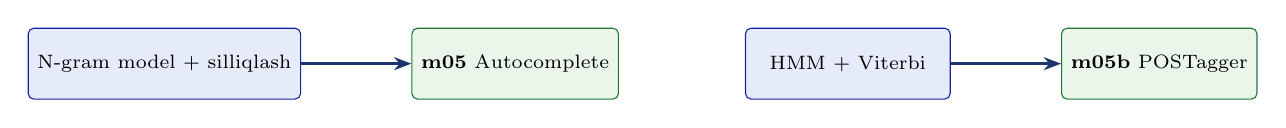
\begin{tikzpicture}[>=Stealth,node distance=8mm]
  \node[wbox,fill=bluebg,draw=mainblue,minimum width=26mm,minimum height=9mm] (ng) {\scriptsize N-gram model $+$ silliqlash};
  \node[wbox,fill=greenbg,draw=ForestGreen,minimum width=24mm,minimum height=9mm,right=14mm of ng] (ac) {\scriptsize\textbf{m05} Autocomplete};
  \node[wbox,fill=bluebg,draw=mainblue,minimum width=26mm,minimum height=9mm,right=16mm of ac] (hmm) {\scriptsize HMM $+$ Viterbi};
  \node[wbox,fill=greenbg,draw=ForestGreen,minimum width=24mm,minimum height=9mm,right=14mm of hmm] (pt) {\scriptsize\textbf{m05b} POSTagger};
  \draw[tran] (ng)--(ac); \draw[tran] (hmm)--(pt);
\end{tikzpicture}}

\vspace{5pt}
\begin{columns}[T,totalwidth=\textwidth]
\begin{column}{0.50\textwidth}
\textbf{5-amaliyotda qurasiz}
\begin{itemize}\setlength\itemsep{3pt}
  \item \texttt{m05 Autocomplete}: bigram $+$ add-1, perplexity;
  \item \texttt{m05b POSTagger}: HMM $+$ \texttt{viterbi};
  \item eng ehtimoliy davom va teg ketma-ketligi.
\end{itemize}
\end{column}

\begin{column}{0.48\textwidth}
\textbf{Birinchi assert} (ushbu ma\uzq{}ruzaning Viterbi slaydi bilan solishtiriladi):

\begin{tcolorbox}[defbox,left=2mm,right=2mm,top=1mm,bottom=1mm]
\begin{verbatim}
assert abs(delta_VB_t2
           - 0.3402) < 1e-4
# yo'l == [NN, VB]
\end{verbatim}
\end{tcolorbox}
\end{column}
\end{columns}

\end{frame}

% ----------------------------------------------------------------
% [Q2] KO'PRIK: 6-MA'RUZAGA (Word2Vec)
% ----------------------------------------------------------------
\begin{frame}{6-ma\uzq{}ruzaga ko\uzq{}prik: N-gram so\uzq{}z ma\uzq{}nosini bilmaydi}
\footnotesize
\begin{columns}[T,totalwidth=\textwidth]
\begin{column}{0.54\textwidth}
N-gram til modeli so\uzq{}zlarni \textbf{alohida (diskret) token} sifatida sanaydi ---
shuning uchun ularning \emph{ma\uzq{}nosini} bilmaydi:
\vspace{3pt}
\begin{tcolorbox}[warnbox,left=2mm,right=2mm,top=1mm,bottom=1mm]
\scriptsize
\texttt{kitob} va \texttt{kitobni}, yoki \texttt{film} va \texttt{kino} --- model uchun
butunlay \textbf{boshqa} tokenlar. Birida o\uzq{}rgangan ehtimol boshqasiga o\uzq{}tmaydi
(ma\uzq{}lumot bo\uzq{}linib ketadi).
\end{tcolorbox}
\end{column}
\begin{column}{0.42\textwidth}
\begin{tcolorbox}[defbox,title=6-ma\uzq{}ruza]
\scriptsize
\textbf{Word2Vec / CBOW:} so\uzq{}zlarni \textbf{zich vektor}ga akslantiradi ---
ma\uzq{}nosi yaqin so\uzq{}zlar (\texttt{film}$\approx$\texttt{kino}) fazoda yaqin,
shuning uchun ma\uzq{}lumot ular orasida \textbf{ulashiladi}.
\end{tcolorbox}
\vspace{3pt}
{\scriptsize\color{halfgray} Ya\uzq{}ni: diskret tokenlardan $\to$ ma\uzq{}noni
ushlaydigan zich vektorlarga.}
\end{column}
\end{columns}
\end{frame}

% ----------------------------------------------------------------
% [R] ADABIYOTLAR
% ----------------------------------------------------------------
\begin{frame}{Adabiyotlar}
\scriptsize

\begin{enumerate}\setlength\itemsep{6pt}
  \item Rabiner, L.R. (1989). \textit{A Tutorial on Hidden Markov Models and Selected
        Applications in Speech Recognition}. Proc. IEEE, 77(2), 257--286.

  \item Jurafsky, D., \& Martin, J. H. (2023).
        \textit{Speech and Language Processing} (3-nashr).
        3-bob: N-gram til modellari; 8-bob: POS va HMM.

  \item Shannon, C. E. (1948).
        \textit{A Mathematical Theory of Communication}.
        Bell System Technical Journal. (Til modellashtirish va entropiya ildizi.)

  \item Chen, S. F., \& Goodman, J. (1999).
        \textit{An Empirical Study of Smoothing Techniques for Language Modeling}.
        Computer Speech \& Language.

  \item \texttt{nltk.lm} hujjatlari --- N-gram til modellari API.
\end{enumerate}

\end{frame}

% ================================================================
% [S] ILOVALAR (appendix --- asosiy slayd soniga kirmaydi)
% ================================================================
\appendix

\begin{frame}{Ilova S1: Log-fazoda Viterbi (amaliy barqarorlik)}
\footnotesize

\begin{columns}[T,totalwidth=\textwidth]
\begin{column}{0.54\textwidth}
\textbf{Logarifmik shakl}
\[
\log\delta_t(j)=\max_i\!\big[\log\delta_{t-1}(i)+\log A(j\mid i)\big]+\log B(o_t\mid j)
\]

\begin{itemize}\setlength\itemsep{3pt}
  \item Ko\uzq{}paytirish $\longrightarrow$ \textbf{qo\uzq{}shish}: kichik ehtimollar
        ko\uzq{}paytmasi o\uzq{}rniga logarifmlar yig\uzq{}indisi $\Rightarrow$ underflow yo\uzq{}q.
  \item $\log$ \textbf{monoton} o\uzq{}suvchi $\Rightarrow$ $\arg\max$ o\uzq{}zgarmaydi:
        orqaga kuzatish (\textit{backtrace}) bir xil yo\uzq{}lni beradi.
\end{itemize}

\vspace{2pt}
\begin{tcolorbox}[okbox,left=2mm,right=2mm,top=1mm,bottom=1mm]
\scriptsize
Misol: $\delta_2(\mathrm{VB})=0.3402$ uchun
$\log\delta_2(\mathrm{VB})=\ln 0.3402\approx -1.078$.
\end{tcolorbox}
\end{column}

\begin{column}{0.46\textwidth}
\centering
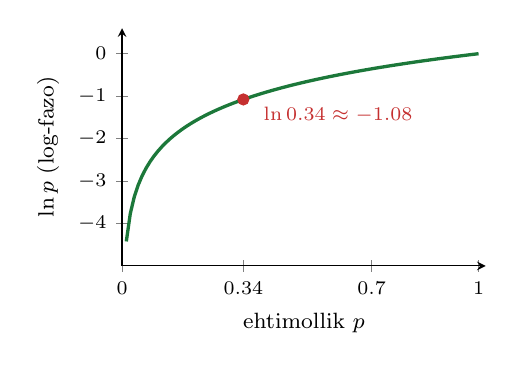
\begin{tikzpicture}
  \begin{axis}[
    width=6.2cm,height=4.6cm,
    xlabel={\footnotesize ehtimollik $p$},
    ylabel={\footnotesize $\ln p$ (log-fazo)},
    xmin=0,xmax=1.02,ymin=-5,ymax=0.6,
    domain=0.012:1,samples=90,
    axis lines=left,tick label style={font=\scriptsize},
    xtick={0,0.3402,0.7,1},xticklabels={$0$,$0.34$,$0.7$,$1$},
    ytick={0,-1,-2,-3,-4},
    enlargelimits=false,clip=false]
    \addplot[ForestGreen,very thick]{ln(x)};
    \addplot[only marks,mark=*,mark size=2pt,HiRed]coordinates{(0.3402,-1.078)};
    \node[anchor=west,font=\scriptsize,HiRed]at(axis cs:0.37,-1.45){$\ln 0.34\approx-1.08$};
  \end{axis}
\end{tikzpicture}\\[-1pt]
{\scriptsize Kichik $p$ $\Rightarrow$ katta manfiy $\log$; tartib saqlanadi.}
\end{column}
\end{columns}

\end{frame}

\begin{frame}{Ilova S2: Perplexity va entropiya bog\uzq{}liqligi}
\footnotesize

\begin{columns}[T,totalwidth=\textwidth]
%------------------------------------------------
\begin{column}{0.50\textwidth}

\textbf{Asosiy bog\uzq{}lanish}

\[
\mathrm{PP}(W)=2^{H(W)}
\]

\[
H(W)=
-\frac1N
\sum_{i=1}^{N}
\log_2 P(w_i\mid w_{i-1})
\]

\vspace{3pt}

\begin{tcolorbox}[defbox,left=2mm,right=2mm,top=1mm,bottom=1mm]
\scriptsize
$H(W)$ — har bir token uchun o\uzq{}rtacha noaniqlik
(\textit{entropy} — entropiya), bitlarda o\uzq{}lchanadi.
\end{tcolorbox}

\vspace{3pt}

\begin{itemize}\setlength\itemsep{4pt}
  \item $H$ kichik bo\uzq{}lsa, model kamroq noaniqlikka ega.
  \item $H$ oshsa, PP ham tez oshadi.
  \item $1$ bit noaniqlik $\Rightarrow 2$ ta teng ehtimolli tanlov.
\end{itemize}

\end{column}

%------------------------------------------------
\begin{column}{0.48\textwidth}
\centering

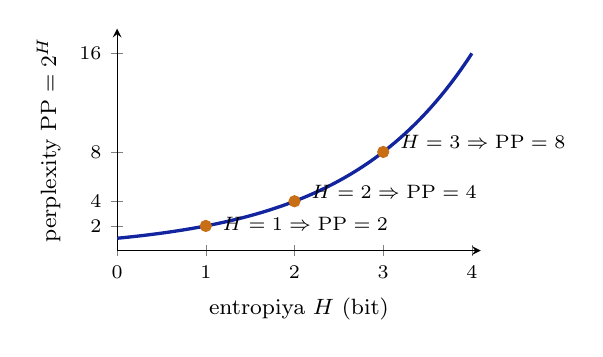
\begin{tikzpicture}
  \begin{axis}[
    width=6.2cm,
    height=4.4cm,
    xlabel={\footnotesize entropiya $H$ (bit)},
    ylabel={\footnotesize perplexity $\mathrm{PP}=2^{H}$},
    xmin=0,xmax=4.1,
    ymin=0,ymax=18,
    domain=0:4,
    samples=70,
    axis lines=left,
    tick label style={font=\scriptsize},
    xtick={0,1,2,3,4},
    ytick={2,4,8,16},
    enlargelimits=false,
    clip=false
  ]
    \addplot[mainblue,very thick]{2^x};

    \addplot[only marks,mark=*,mark size=2pt,VBc]
      coordinates{(1,2)(2,4)(3,8)};

    \node[anchor=west,font=\scriptsize] at (axis cs:1.08,2.2)
      {$H=1 \Rightarrow \mathrm{PP}=2$};

    \node[anchor=west,font=\scriptsize] at (axis cs:2.08,4.8)
      {$H=2 \Rightarrow \mathrm{PP}=4$};

    \node[anchor=west,font=\scriptsize] at (axis cs:3.08,8.8)
      {$H=3 \Rightarrow \mathrm{PP}=8$};
  \end{axis}
\end{tikzpicture}

\vspace{3pt}

\begin{tcolorbox}[okbox,left=2mm,right=2mm,top=1mm,bottom=1mm]
\scriptsize
Entropiya chiziqli oshsa, perplexity eksponensial oshadi.
Shuning uchun past entropiya va past PP yaxshi model belgisi.
\end{tcolorbox}

\end{column}
\end{columns}

\end{frame}

\end{document}
